%===============================================================================
% LaTeX sjabloon voor de bachelorproef toegepaste informatica aan HOGENT
% Meer info op https://github.com/HoGentTIN/bachproef-latex-sjabloon
%===============================================================================

\documentclass{bachproef-tin}
\usepackage{hogent-thesis-titlepage} % Titelpagina conform aan HOGENT huisstijl
\usepackage{biblatex}
\addbibresource{bachproef-tin.bib}

%%---------- Documenteigenschappen ---------------------------------------------
% TODO: Vul dit aan met je eigen info:

% De titel van het rapport/bachelorproef
\title{Technieken en methodieken om AI en AR toe te passen bij de optimalisatie van Wayfinding: een vergelijkende studie en proof-of-concept}

% Je eigen naam
\author{Rob De Putter}

% De naam van je promotor (lector van de opleiding)
\promotor{Steven Van Impe}

% De naam van je co-promotor. Als je promotor ook je opdrachtgever is en je
% dus ook inhoudelijk begeleidt (en enkel dan!), mag je dit leeg laten.
\copromotor{Thijs Morlion}

% Indien je bachelorproef in opdracht van/in samenwerking met een bedrijf of
% externe organisatie geschreven is, geef je hier de naam. Zoniet laat je dit
% zoals het is.
\instelling{In The Pocket}

% Academiejaar
\academiejaar{2019-2020}

% Examenperiode
%  - 1e semester = 1e examenperiode => 1
%  - 2e semester = 2e examenperiode => 2
%  - tweede zit  = 3e examenperiode => 3
\examenperiode{2}

%===============================================================================
% Inhoud document
%===============================================================================

\begin{document}

%---------- Taalselectie -------------------------------------------------------
% Als je je bachelorproef in het Engels schrijft, haal dan onderstaande regel
% uit commentaar. Let op: de tekst op de voorkaft blijft in het Nederlands, en
% dat is ook de bedoeling!

%\selectlanguage{english}

%---------- Titelblad ----------------------------------------------------------
\inserttitlepage

%---------- Samenvatting, voorwoord --------------------------------------------
\usechapterimagefalse
%%=============================================================================
%% Voorwoord
%%=============================================================================

\chapter*{\IfLanguageName{dutch}{Woord vooraf}{Preface}}
\label{ch:voorwoord}

%% TODO:
%% Het voorwoord is het enige deel van de bachelorproef waar je vanuit je
%% eigen standpunt (``ik-vorm'') mag schrijven. Je kan hier bv. motiveren
%% waarom jij het onderwerp wil bespreken.
%% Vergeet ook niet te bedanken wie je geholpen/gesteund/... heeft
Dit eindwerk vormt de afsluiter van mijn professionele bacheloropleiding Toegepaste Informatica, afstudeerrichting Mobiele Applicaties aan de HoGent. Ik kan terug kijken naar 3 fantastische jaren waar ik zeer veel heb bijgeleerd en veel nieuwe vrienden heb gemaakt.

Het onderzoek dat werd uitgevoerd in deze bachelorproef gaat vooral over Artificiële intelligentie, een domein binnen informatica dat in onze opleiding alleen op theoretisch vlak werd aangeboden. Om mijn kennis te verrijken en wat meer te verdiepen in welke mogelijkheden er zijn met deze technologie heb ik ervoor gekozen om dit te betrekken in het afsluitende opleidingsonderdeel. Ik ben een student die ernaar streeft om relevante technologieën te begrijpen en mogelijks ook te gebruiken in projecten. Alsook probeer ik zoveel mogelijk unieke ervaringen op te doen, in het laatste semester van mijn bachelor heb ik er dan ook voor gekozen om mijn studies in het buitenland af te ronden door middel van een buitenlandse stage. Dit aspect heeft zeker een effect gehad op het uitwerken van dit onderzoek, ik had veel minder resources ter beschikking, maar ze hebben me altijd geleerd om te roeien met de riemen die je hebt.
Uit het onderzoek dat ik heb uitgevoerd heb ik zeker bijgeleerd, ik ben veel meer op de hoogte van welke AI-eigenschappen een AI-framework te bieden heeft.

Het eindresultaat van deze bachelorproef zou nooit hetzelfde zijn zonder de hulp van mijn promotor Steven Van Impe en co-promotor Thijs Morlion, zij hebben mijn eindwerk zorgvuldig nagelezen en tips gegeven waar het nodig was. Ik wel hen beiden dan ook ten zeerste bedanken. Alsook wil ik mijn zus, Lise De Putter bedanken, zij heeft deze bachelorproef meerdere malen nagelezen om alle punten op i te zetten.

\newpage
Veel appreciatie ben ik ook verschuldigd aan alle docenten en begeleiders van mijn opleiding Toegepaste Informatica, zij zijn elke dag in de weer om alle studenten op te leiden tot IT-professionals, wat geen makkelijke zaak is. Zij gaven mij ook meer toekomstperspectief en motivatie om zoveel mogelijk bij te leren.

Een speciaal woordje van dank gaat uit naar mijn dierbare vrienden en studiegenoten die mij altijd hebben gesteund tijdens moeilijke (en gewone) tijden. Zonder hen zou deze opleiding nooit hetzelfde zijn geweest.

Ik wens u veel leesplezier toe.

Rob De Putter

Kerksken, 25 mei 2020



%%=============================================================================
%% Samenvatting
%%=============================================================================

% TODO: De "abstract" of samenvatting is een kernachtige (~ 1 blz. voor een
% thesis) synthese van het document.
%
% Deze aspecten moeten zeker aan bod komen:
% - Context: waarom is dit werk belangrijk?
% - Nood: waarom moest dit onderzocht worden?
% - Taak: wat heb je precies gedaan?
% - Object: wat staat in dit document geschreven?
% - Resultaat: wat was het resultaat?
% - Conclusie: wat is/zijn de belangrijkste conclusie(s)?
% - Perspectief: blijven er nog vragen open die in de toekomst nog kunnen
%    onderzocht worden? Wat is een mogelijk vervolg voor jouw onderzoek?
%
% LET OP! Een samenvatting is GEEN voorwoord!

%%---------- Nederlandse samenvatting -----------------------------------------
%
% TODO: Als je je bachelorproef in het Engels schrijft, moet je eerst een
% Nederlandse samenvatting invoegen. Haal daarvoor onderstaande code uit
% commentaar.
% Wie zijn bachelorproef in het Nederlands schrijft, kan dit negeren, de inhoud
% wordt niet in het document ingevoegd.

\IfLanguageName{english}{%
\selectlanguage{dutch}
\chapter*{Samenvatting}
\lipsum[1-4]
\selectlanguage{english}
}{}

%%---------- Samenvatting -----------------------------------------------------
% De samenvatting in de hoofdtaal van het document

\chapter*{\IfLanguageName{dutch}{Samenvatting}{Abstract}}

Artificiële Intelligentie (AI) en Augmented Reality (AR) zijn bijna niet meer weg te denken binnen de IT-wereld. De laatste jaren kenden beide technologieën een groei dankzij hun vooruitgang, zo werden deze technologieën accurater en performanter. AR werd geïntroduceerd op sociale media door middel van Snapchat -en Instagramfilters, ook Pokemon Go maakt gebruik van deze technologie. AI bestaat reeds langer, één van de bekendste hulpmiddelen die gebruik maken van deze technologie zijn Google Home, Alexa en Siri. 

In deze bachelorproef zullen deze twee technologieën gecombineerd worden om een indoor wayfinding applicatie te optimaliseren. Wayfinding kan je verstaan als het denkvermogen dat nodig is om de weg terug te vinden in een specifieke omgeving. Deze applicatie zal de gebruiker de weg wijzen met behulp van 3D-pijlen die op het mobiele toestel zullen verschijnen, hier wordt AR geïntroduceerd in het verhaal. AR zal ervoor zorgen dat de 3D-pijlen op een gepaste manier worden getoond. Het bepalen hoe de pijlen worden getoond op het scherm is van cruciaal belang, het is zeer belangrijk dat deze zich bijvoorbeeld niet door muren begeven. Daarom is het belangrijk dat de omgeving op een zo goed mogelijke manier in kaart wordt gebracht. Het in kaart brengen van de omgeving is een aspect dat reeds wordt gedaan door AR, maar dit kan geoptimaliseerd worden door AI. Artificiële intelligentie zal bijvoorbeeld de muren van het grondoppervlak kunnen onderscheiden, waardoor dergelijke fouten niet meer zullen voorkomen.

In dit onderzoek werd bestudeerd welke mogelijke AI-frameworks in staat zijn om dergelijke zaken uit te voeren, vervolgens werden een paar van deze frameworks getest en geëvalueerd op basis van beoordelingstechnieken die de verschillende noden van een wayfinding applicatie nastreven. Deze frameworks werden tegenover elkaar gezet en diegene met de beste resultaten werd verkozen als 'eindwinnaar'.

Door de beperkte middelen tijdens het uitvoeren van dit onderzoek kan deze bachelorproef zeker nog worden geoptimaliseerd. In het vervolg op deze bachelorproef kunnen proeven op een grootschaligere manier worden uitgevoerd. Het framework met de beste resultaten zou ook in een praktisch voorbeeld kunnen worden uitgewerkt.



%---------- Inhoudstafel -------------------------------------------------------
\pagestyle{empty} % Geen hoofding
\tableofcontents  % Voeg de inhoudstafel toe
\cleardoublepage  % Zorg dat volgende hoofstuk op een oneven pagina begint
\pagestyle{fancy} % Zet hoofding opnieuw aan

%---------- Lijst figuren, afkortingen, ... ------------------------------------

% Indien gewenst kan je hier een lijst van figuren/tabellen opgeven. Geef in
% dat geval je figuren/tabellen altijd een korte beschrijving:
%
%  \caption[korte beschrijving]{uitgebreide beschrijving}
%
% De korte beschrijving wordt gebruikt voor deze lijst, de uitgebreide staat bij
% de figuur of tabel zelf.

\listoffigures
\listoftables

% Als je een lijst van afkortingen of termen wil toevoegen, dan hoort die
% hier thuis. Gebruik bijvoorbeeld de ``glossaries'' package.
% https://www.overleaf.com/learn/latex/Glossaries

%---------- Kern ---------------------------------------------------------------

% De eerste hoofdstukken van een bachelorproef zijn meestal een inleiding op
% het onderwerp, literatuurstudie en verantwoording methodologie.
% Aarzel niet om een meer beschrijvende titel aan deze hoofstukken te geven of
% om bijvoorbeeld de inleiding en/of stand van zaken over meerdere hoofdstukken
% te verspreiden!
%%=============================================================================
%% Inleiding
%%=============================================================================
\chapter{\IfLanguageName{dutch}{Inleiding}{Introduction}}
\label{ch:inleiding}

\section{\IfLanguageName{dutch}{Wayfinding}{Wayfinding}}
\label{sec:wayfinding}
Het begrip ''Wayfinding'' is op zich zeer breed, algemeen staat het gekend als het gedrag en denkvermogen dat nodig is om de weg terug te vinden in een specifieke omgeving. Om zich te verplaatsen heeft men reeds smartphones en GPS-implementaties, wayfinding zit hier dus ook in verweven. In deze bachelorproef zal men bespreken hoe men wayfinding op een optimale manier kan toepassen met behulp van technische middelen.

\section{\IfLanguageName{dutch}{Probleemstelling}{Problem Statement}}
\label{sec:probleemstelling}

In The Pocket is een Belgisch IT-bedrijf dat zich focust op digitale producten, zij wensen een GPS-applicatie te implementeren dat wayfinding optimaliseert, dit betekent dat er geen fouten meer worden gemaakt bij het wijzen van de weg. Om deze toepassing te optimaliseren verlangt men gebruik te maken van AI en AR om omgevingsfactoren te detecteren, te analyseren en bovendien de input te vertalen naar de AR-omgeving. Als men bijvoorbeeld tegen een muur dreigt te lopen, dan kan AI dit corrigeren. In deze bachelorproef zal ik een onderzoek voeren dat resulteert in een overzicht van verschillende mogelijke algoritmes en/of aanpakken. Deze zal men kunnen toepassen bij het implementeren van de gewenste GPS-applicatie.

\section{\IfLanguageName{dutch}{Onderzoeksvraag}{Research question}}
\label{sec:onderzoeksvraag}

\subsection{Hoofdvraag}
Welke bestaande technieken bestaan er reeds om aan de hand van AI en AR de drift in wayfinding te optimaliseren? Hoe kunnen we de wereld rondom de gebruiker herkennen, analyseren en bovendien de input op een bruikbare manier vertalen naar de AR-omgeving?

\subsection{Deelvraag}
Wat is het optimale algoritme/techniek om de drift in wayfinding te optimaliseren aan de hand van AI en AR? 

\section{\IfLanguageName{dutch}{Onderzoeksdoelstelling}{Research objective}}
\label{sec:onderzoeksdoelstelling}

De doelstelling van dit onderzoek is om een duidelijk overzicht te creëren van welke algoritmes en/of aanpakken goede prestaties zullen leveren bij het implementeren in de wayfinding context. Goede prestaties kan men vertalen in een applicatie (proof-of-concept) die zonder fouten, de juiste route zal aangeven.
De ultieme succesfactor van deze bachelorproef is het vinden van één of meerdere algoritmen die het bedrijf ''In The Pocket'' zou kunnen gebruiken bij het implementeren van de concrete GPS-applicatie.



\section{\IfLanguageName{dutch}{Opzet van deze bachelorproef}{Structure of this bachelor thesis}}
\label{sec:opzet-bachelorproef}

% Het is gebruikelijk aan het einde van de inleiding een overzicht te
% geven van de opbouw van de rest van de tekst. Deze sectie bevat al een aanzet
% die je kan aanvullen/aanpassen in functie van je eigen tekst.

De rest van deze bachelorproef is als volgt opgebouwd:

In Hoofdstuk~\ref{ch:stand-van-zaken} wordt een overzicht gegeven van de stand van zaken binnen het onderzoeksdomein, op basis van een literatuurstudie.

In Hoofdstuk~\ref{ch:methodologie} wordt de methodologie toegelicht en worden de gebruikte onderzoekstechnieken besproken om een antwoord te kunnen formuleren op de onderzoeksvragen.

% TODO: Vul hier aan voor je eigen hoofstukken, één of twee zinnen per hoofdstuk

In Hoofdstuk~\ref{ch:conclusie}, tenslotte, wordt de conclusie gegeven en een antwoord geformuleerd op de onderzoeksvragen. Daarbij wordt ook een aanzet gegeven voor toekomstig onderzoek binnen dit domein.
\chapter{\IfLanguageName{dutch}{Stand van zaken}{State of the art}}
\label{ch:stand-van-zaken}

% Tip: Begin elk hoofdstuk met een paragraaf inleiding die beschrijft hoe
% dit hoofdstuk past binnen het geheel van de bachelorproef. Geef in het
% bijzonder aan wat de link is met het vorige en volgende hoofdstuk.

% Pas na deze inleidende paragraaf komt de eerste sectiehoofding.


In dit deel zal men toespitsen op de werking van een wayfinding applicatie, bij uitstek de concrete werking van het AI/AR mechanisme.

\section{Begrippen}
\subsection{AI (Artificiële intelligentie)}
Artificiële intelligentie of AI is een zeer groot fenomeen in de huidige IT-wereld. Men kan het beschrijven als intelligentie die wordt gedemonstreerd door machines. Op deze manier kunnen die apparaten de omgeving waarnemen en vervolgens acties ondernemen die het succesvol bereiken van een bepaald doel zal maximaliseren. In het algemeen staat de term AI ook gekend als de beschrijving van machines of computers die cognitieve acties uitvoeren die wij als mensen associeren met de menselijke geest. 

In deze bachelorproef wordt AI toegepast op het vlak van objectdetectie, het is de meest cruciale factor om een wayfinding applicatie te optimaliseren.
Objectdetectie zal in de wayfinding applicatie er voor zorgen dat de omgeving op een correcte manier wordt herkend, zo kan men een perfect beeld scheppen van welke objecten men afstand moet houden, bijvoorbeeld muren.

\subsubsection{Objectherkenning vs. Objectdetectie}
In Artificiële intelligentie heeft men twee verschillende manieren om objecten te identificeren, objectherkenning en objectdetectie. Het herkenningsproces is zeer gelijkaardig, maar toch zijn er zekere verschillen bij de uitvoering. Objectdetectie kan men beschouwen als een subset van objectherkenning, men zal de objecten herkennen op een simultane manier, maar bij objectdetectie wordt het object ook gelocaliseerd in de afbeelding. In de onderstaande afbeelding kan men het verschil duidelijk waarnemen, objectherkenning (links) en objectdetectie (rechts).

\begin{center}
	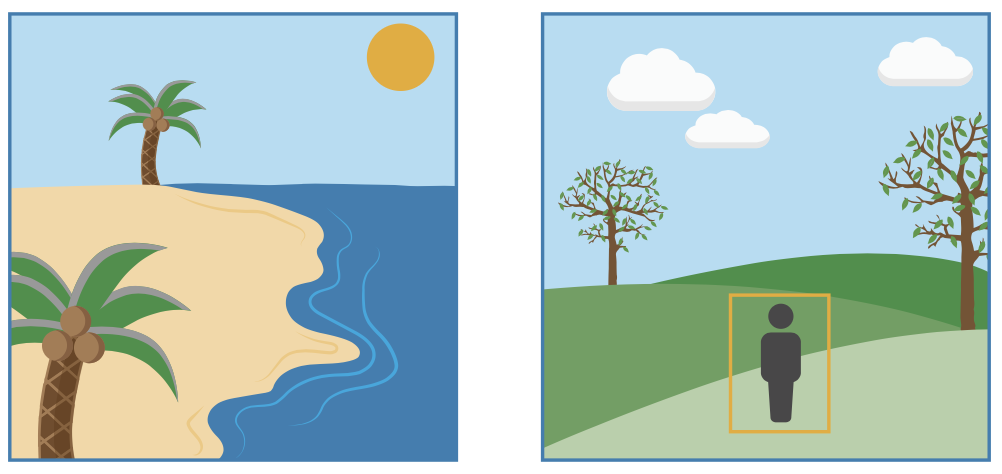
\includegraphics[scale=0.35]{objectdetectie.png}
\end{center}

\subsection{Werking van objectherkenning}
Om objectherkenning toe te passen kan je gebruik maken van twee verschillende manieren, namelijk 'Machine Learning' en 'Deep learning'. Beide technieken zullen objecten gaan herkennen, maar ze zijn verschillend op vlak van uitvoering.

\subsubsection{Machine learing}
Machine learning maakt gebruik van classificatie om een bepaald object te herkennen. Ten eerste zal men een trainingset opstellen, dit gebeurt door een verzameling van afbeeldingen samen te stellen en vervolgens de relevante punten aan te duiden. Het is zeer belangrijk om de juiste relevante punten aan te duiden, anders zal het systeem verkeerd getraind worden, waardoor men vervolgens een verkeerde output zal verkrijgen. Deze punten zullen er voor zorgen dat het systeem verschillende categorieën herkent. Vervolgens zal het leermodel deze informatie gebruiken om nieuwe objecten (objecten die nog niet gekend zijn in de trainingset) te analyseren en te classificeren.

\begin{center}
	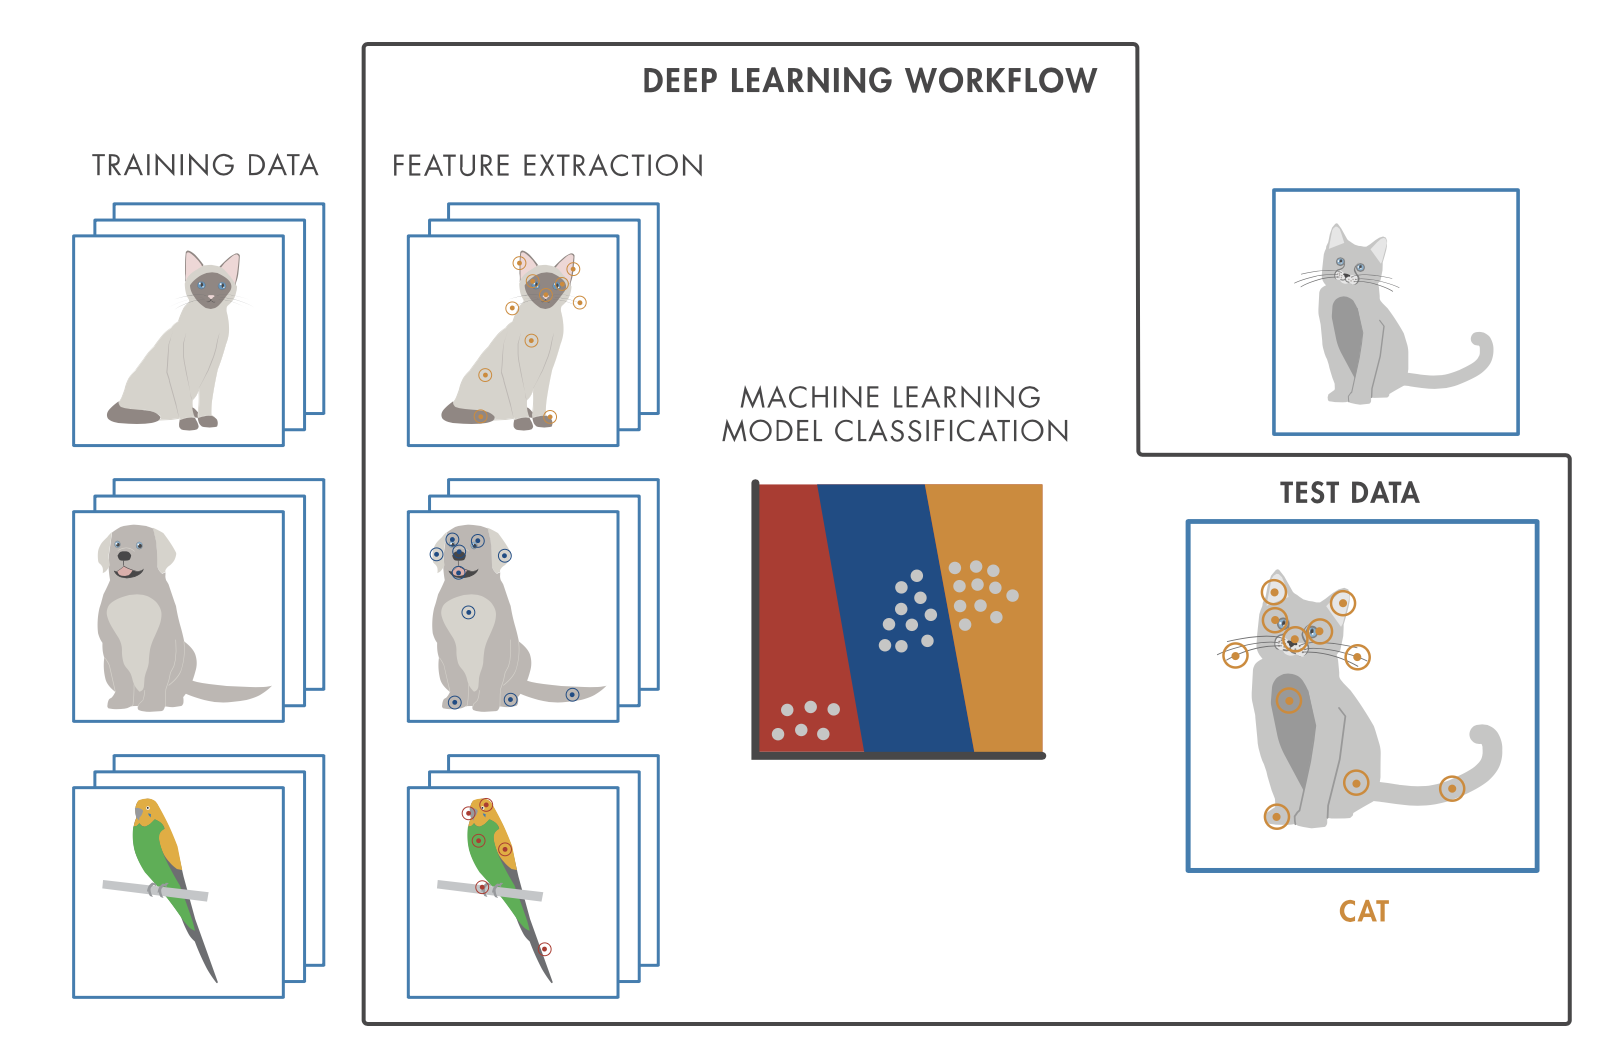
\includegraphics[scale=0.4]{machinelearning.png}
\end{center}

\subsubsection{Deep learning}
Deep learning maakt gebruik van convulationele neurale netwerken (CNN) om objecten te herkennen. Een CNN kan automatisch de aanhangende kenmerken van een object leren om dat object te identificeren, dit betekent dat een CNN bijvoorbeeld het verschil tussen auto's en vrachtwagens kan herkennen door middel van duizenden afbeeldingen te analyseren en vervolgens te leren welke kenmerken juist verschillend zijn.

\begin{center}
	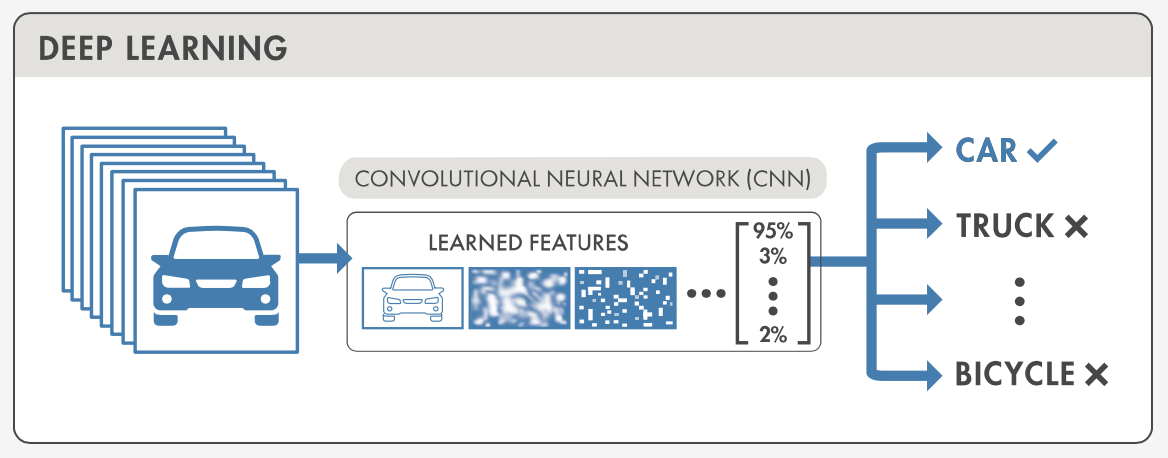
\includegraphics[scale=0.47]{deeplearning.png}
\end{center}

\subsection{AR (Augmented reality)}
Het concept AR is vandaag de dag niet meer uit het straatbeeld weg te denken, het wordt bijvoorbeeld gebruikt bij de Instagram -en Snapchat filters. Augmented reality of AR is een interactieve ervaring met de omgeving waarin objecten die zich in de echte wereld bevinden worden versterkt door computergegenereerde objecten. AR is iets wat al even bestaat, het werd bijvoorbeeld al gebruikt bij één van de eerste straaljagers, het visier van de piloot wordt in dit voorbeeld ondersteund door een computergegenereerd object dat de vijand zou moeten lokaliseren. Augmented reality werd pas populair bij de modale mens wanneer Naintic Pokemon Go lanceerde, het werd één van de meest gekende smarthonegames. In 2017 introduceerde Android en Apple, AR Core en AR Kit, het werd vervolgens voor developers veel eenvoudiger om AR-applicaties te creëren.

Het doel van Augemented reality in deze bachelorproef is om de route op een zo efficiënt mogelijke manier aan te geven, dit betekent dat er geen pijlen door objecten mogen gaan. Om een beeld te kunnen scheppen over het effectieve doeleinde, heeft men alvast een voorbeeldfoto toegevoegd.

\begin{center}
	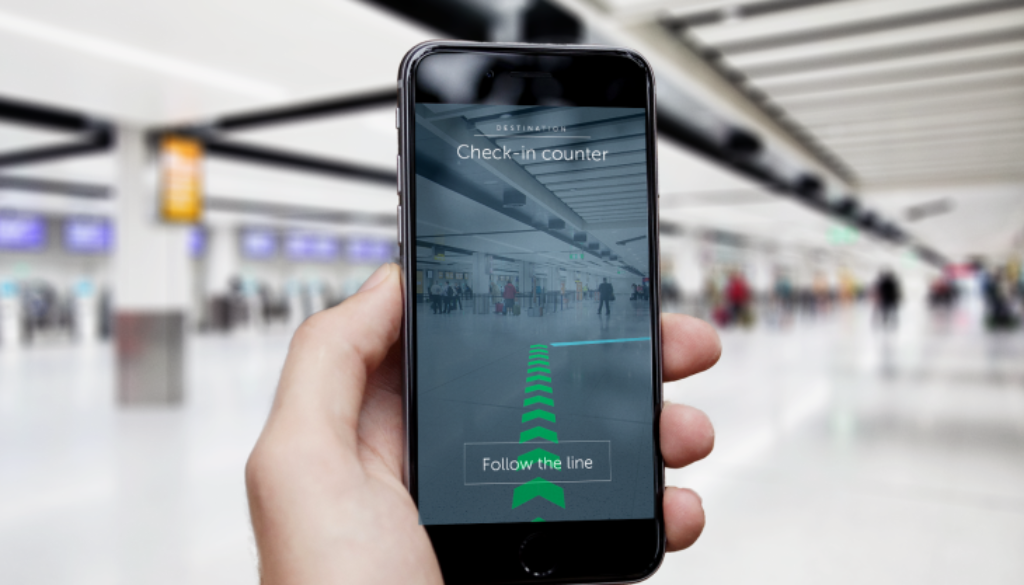
\includegraphics[scale=0.25]{wayfinding.png}
\end{center}

\subsection{Werking van Augmented realtiy}
Augmented reality kan momenteel op drie verschillende manieren worden uitgewerkt, namelijk door middel van SLAM, herkenning gebaseerd en locatie gebaseerd.

\subsubsection{SLAM (Simultaneous Localization and Mapping)}
Simultaneous Localization and Mapping of SLAM is de manier die het meest effectief en efficiënt werkt. SLAM lokaliseert sensoren ten opzichte van hun omgeving en brengt tegelijkertijd de omgeving in kaart, het is dus een zeer goede aanpak om complexe AR-simulatieproblemen op te lossen. Het SLAM-systeem is in feite een set van algoritmen die gericht zijn op het oplossen van gelijktijdige lokalisatie en het in kaart brengen van problemen. De meeste Augmented realitykits zijn reeds uitgerust met de mogelijkheid tot een SLAM-aanpak.

\subsubsection{Herkenning gebaseerd}
Herkenning gebaseerd gebruikt de camera van het gebruikte apparaat om bepaalde visuele markers of objecten te identificeren. Deze AR-technologie is bijgevolg zeer afhankelijk van de kwaliteit van de gebruikte camera, als deze de markers niet goed kan identificeren, dan zal het AR mechanisme niet goed werken.

Bij deze manier is het ook mogelijk om de positie en oriëntatie te berekenen. De markers op het scherm worden vervangen door een overeenkomstig 3D-object, dit maakt het mogelijk om het object meer in detail te bekijken door het bijvoorbeeld te roteren zodat men meerdere invalshoeken kan observeren.

\subsubsection{Locatie gebaseerd}
Locatie gebaseerd of 'markerless augmented reality' is een AR-technologie die alleen gebruikt maakt van een GPS, digitaal kompas, snelheidsmeter of versnellingsmeter om gegevens over de locatie te verzamelen, de augmented reality visualisaties worden met behulp van deze informatie geactiveerd. Een smartphone heeft genoeg sensoren om deze manier te kunnen realiseren. 

\subsection{AI + AR}
De samenhang van Artificiële intelligentie en Augmented reality is zeer cruciaal bij het optimaliseren van een wayfinding applicatie. Ten eerste is het belangrijk dat de objecten op een correcte manier worden herkend. Ten tweede is het zeer belangrijk dat de bevindingen van de objectherkenning op een correcte manier worden vertaald naar de AR omgeving. 

\section{Literatuurstudie}

In deze sectie zal men meer focussen op het onderzoek en de uitwerkingen die reeds werden gerealiseerd. Men zal deze algemene kennis kunnen gebruiken om mijn onderzoek te ondersteunen. Deze literatuurstudie staat ook in thema met de wayfinding-context, op deze manier is de verkregen informatie relevanter.

In het algemeen kan ik op voorhand al besluiten dat er reeds weinig onderzoek is gedaan naar de samenhang van 'Artificiële intelligentie' en 'Augemented reality' binnen de wayfinding-context. De termen AI en AR zijn afzondelijk van elkaar zeer gekend in de IT-wereld, men kan dit zelfs niet meer uit het straatbeeld wegdenken. Door de grote belangstelling voor AI en AR, en de minieme huidige onderzoekstoestand binnen de wayfinding-context wordt deze bachelorproef alleen maar interessanter.

\subsection{Artificiële intelligentie (AI)}

\subsubsection{Objectherkenning}
In het uitgave van ~\autocite{Liang2015}, \textcite{Liang2015} werd er onderzoek gedaan naar het gebruik van objectherkenning door middel van 'Convolutionele netwerken' of met andere woorden, 'Deep learning'. De auteurs werden geïnspireerd door 'Deep learning' omdat het reeds meerdere successen had geboekt bij andere computervisietaken. Omdat objectherkenning een zeer belangrijk factor is voor veel complexe systemen, wouden ze dit efficiënter maken en dus ook verbeteren, en dit door gebruik te maken van een geanvanceerde techniek, namelijk de convolutionele netwerken. 

Tijdens hun onderzoek werd het netwerk getest door middel van meerdere datasets, namelijk CIFAR-10, CIFAR-100, MNIST en SVHN. Deze datasets zijn zeer handig wanneer men convolutionele netwerken wilt testen, men hoeft dus geen data meer te verzamelen om te kunnen observeren of een netwerk wel degelijk goed functioneert. Het vinden van goede datasets is een cruciale factor bij het gebruik van AI, indien deze niet voldoen aan de eisen kan men ook geen bruikbare conclusies opstellen.

In het onderzoek verduidelijkt men ook nog eens het gebruik van 'Deep learning' zorgt voor betere resultaten. Het verhogen van de parameters in een CNN zorgde in het onderzoek voor nog een betere performantie, in tegenstelling met de 'gewone' feed-forward structuur. 

Uit de conclusie van hun onderzoek kan men besluiten dat een RCNN (recurrent convolutioneel netwerk) betere resultaten opleverd. Een recurrent convolutioneel netwerk is uitgebreider CNN, men gaat meer recurrente verbindingen (of parameters) toevoegen in elke laag. Deze structuur maakte het mogelijk om meer diepgang te creëren, men ging met andere woorden meer informatie verkrijgen uit elke laag, waardoor men meer kans kreeg op het juist eindresultaat. In de laatste fase van het onderzoek kon men andermaal besluiten dat het netwerk nog efficiënter werkte, bij het toevoegen van (nog) meer parameters.


Objectherkenning kan ook rechtstreeks gebruikt worden om de juiste weg te berekenen, dit wordt aangetoond in de studie van \autocite{Haikun2017}. In deze paper werd een wayfinding-ontwerp voor een virtuele wereld geoptimaliseerd. Vroeger werd een wayfinding-ontwerp handmatig opgesteld, hierbij moest men rekening houden met talloze verschillende parameters die mogelijks kunnen veranderen. Zo is het mogelijk dat de menselijke factoren als omgevingsfactoren  kunnen veranderen, een statisch ontwerp creëren die steeds voldoet aan relevante eisen is dus niet haalbaar.

Om dit probleem op te lossen werd 'Way to Go!' gecreërd, dit is een systeem dat automatisch een dynamisch wayfinding-ontwerp kan genereren voor verschillende navigatiemogelijkheden. Het systeem werkt als volgt. Ten eerste moet men een navigatiescenario specifiëren, met moet met andere woorden een route uitstippelen. Ten tweede zal het systeem automatisch een geoptimaliseerd wayfinding-ontwerp creëren met borden die op de juiste manier zijn geplaatst, rekening houdend met de zichtbaarheid van menselijke agenten en de mogelijkheid om fouten te maken tijdens een navigatie.  In het onderzoek evalueert men de resultaten door verschillende wayfinding-ontwerpen te vergelijken en laten zien dat het geoptimaliseerde wayfinding-ontwerp voetgangers effectief en efficiënt naar hun bestemming kan leiden. De aanpak kan de ontwerper van het ontwerp ook helpen om de bereikbaarheid van een bestemming vanaf verschillende locaties te visualiseren en eventuele "blinde" zones te corrigeren met extra bewegwijzering.

\subsubsection{Postionering}
 
\subsection{Augmented reality (AR)}

\subsubsection{Simultaneous Localization and Mapping (SLAM)}
Het onderzoek van \autocite{Zhang2017} heeft als hoofddoel om het leven voor slechtzienden makkelijk te maken. Men wenst dit doel te bereiken met behulp van een indoor wayfinding applicatie te creëren die deze bepaald groep mensen zal begeleiden bij het vinden van de weg, specifiek in gebouwen. Dit onderzoek is zeer vergelijkbaar met deze bachelorproef, het eindproduct kent bijna een grote gelijkenis, alleen wordt er in deze paper gebruik gemaakt van audio-ondersteuning. Men is er dan ook van overtuigt dat deze publicatie zal helpen bij het vinden van het gepaste eindresultaat.

In dit onderzoek probeert men huidige SLAM-technieken te verbeteren, volgens de state-of-the-art werden er steeds fouten bevonden bij het bepalen van de correcte positie, de zogekende 6-DOF-fout. De gekende aanpassingen die werden toegepast tijdens het onderzoek verbeterden niet alleen de 6-DOF-fout, maar ook de rekentijd. Dit resulteert in een snellere response naar de eindgebruiker, wat alleen maar een positieve invloed heeft op de gebruiksvriendelijkheid. In het onderzoek werden ook experimenten uitgevoerd, deze toonden daadwerkelijk aan dat de effectiviteit van het navigeren wel degelijk werd verbeterd voor slechtziende mensen.

\subsection{Artificiële intelligentie (AI) + Augmented reality (AR)}
Die paper van \autocite{Pouria2016} zal zeer veel hulp bieden, het eindresultaat van dit onderzoek kent namelijk een zeer grote overeenkomst met de objectieven van deze bachelorproef. Dit onderzoek gebruikt evenals hetzelfde soort toestel om te communiceren met de gebruiker.

In de uitwerking hield men rekening met de sensoren die men kan vinden in mobiele toestellen, hiermee ging men ook aan de slag. Deze sensoren hebben het mogelijk gemaakt om de locatie, koers en oriëntatie van de gebruiker te detecteren en om contextuele informatie uit verschillende bronnen van online gegevens te verkrijgen. Het combineren van de verkregen data van positionerings- en oriëntatiesensoren met camera's heeft het ook mogelijk gemaakt om praktische Augmented Reality (AR)-toepassingen op deze mobiele apparaten in te zetten. 

Voor de uitwerking van de paper werd een systeem gecreëerd dat een beeld geeft over de navigatiebeleving, dit werd gerealiseerd door middel van Augmented reality en continue feedback van de gebruiker ten opzichte van de dichtsbijzijnde oriëntatiepunten. Deze oriëntatiepunten zijn nodig voor de navigatie en om het juiste pad te vinden. De exacte positie werd bepaald door middel van GPS-sensoren, deze zijn reeds aanwezig in mobiele apparaten. Bovenop de GPS-data werd ook gebruik gemaakt van een beeldverwerkingsalgoritme die de juiste afstand berekent tot een oriëntatiepunt.Om de effectiviteit van het padvinden te verbeteren werd een machinaal leeralgoritme toegevoegd. Dit algoritme zal er voor zorgen dat men voor elke gebruiker een bewegingsprofiel kan opstellen, dit profiel zal er voor zorgen dat men steeds aanpassingen kan uitvoeren op de navigatie-instructies.

Uit de experimenten werd gebleken dat het gebruikte algoritme veel betere resultaten leverde als een 'normaal' turn-by-turn systeem, deze technologie wordt gebruikt bij de huidige GPS-toestellen.


%%=============================================================================
%% Methodologie
%%=============================================================================

\chapter{\IfLanguageName{dutch}{Methodologie}{Methodology}}
\label{ch:methodologie}

%% TODO: Hoe ben je te werk gegaan? Verdeel je onderzoek in grote fasen, en
%% licht in elke fase toe welke stappen je gevolgd hebt. Verantwoord waarom je
%% op deze manier te werk gegaan bent. Je moet kunnen aantonen dat je de best
%% mogelijke manier toegepast hebt om een antwoord te vinden op de
%% onderzoeksvraag.

In dit stuk van de bachelorproef zal men uitleggen hoe het onderzoek tot stand heeft gebracht. Men kan hierin waarnemen hoe men beslissingen heeft genomen omtrent specifieke eigenschappen van de verschillende AI-frameworks. Dit hoofdstuk is verdeeld is vier subsecties, elk van hen verdiept zich meer in hoe elk bepaald stuk van het onderzoek werd gerealiseerd.

\section{Voorbereiding}
Deze subsectie verdiept zich in hoe het toekomstig onderzoek werd uitgestippeld. Men ging verschillende toenaderingen zoeken om een AI-framework op een zo goed mogelijke manier te kunnen evalueren, dit is vervolgens het raamwerk dat werd gebruikt als aanpak in de evaluatie. Er werd ook een extra exploratief onderzoek verwezenlijkt om reeds uitgewerkte voorbeelden te achterhalen die gebruikt maakten van de concrete AI-frameworks. Op deze manier kon men snel testen of de frameworks de moeite waard zijn om deze verder te gebruiken in de proof-of-concept.
\newpage

\subsection{ Onderzoek naar AI-frameworks}
Bij het zoeken van de verschillende frameworks heeft men rekening gehouden met bepaalde criteria die invloed zouden kunnen hebben op het onderzoek:
\begin{itemize}
	\item De kost van het framework (betalend of gratis)
	\item Een mogelijke limiet op het aantal 'calls'
	\item De compatibiliteit met ARKit
	\item Documentatie
	\item Reeds uitgewerkte voorbeelden
\end{itemize}

In dit onderzoek werden 2 AI-frameworks onder de loep genomen, deze voldeden reeds aan alle criteria die werden opgesteld:

\begin{itemize}
	\item TensorFlow Lite (TensorFlow)
	\item CoreML (Apple)
\end{itemize}

De twee andere frameworks die ook werden besproken in de stand van zaken werden niet onderzocht, deze frameworks zijn immers betalend (Vuforia en Vision API). 

\subsection{Beoordelingstechnieken}
Om het juiste AI-framework te kiezen heeft men elk van hen op een grondige manier geëvalueerd. Om dit op een optimale manier te doen heeft men rekening gehouden met verschillende beoordelingstechnieken.

\subsubsection{Functionaliteit}
De eerste factor waar men rekening mee heeft gehouden is het feit of het AI-framework wel degenlijk deed wat er gevraagd werd. Om de frameworks op een zo divers mogelijk manier te kunnen testen heeft men verschillende soorten AI-eigenschappen getest:
\begin{itemize}
	\item Objectdetectie
	\item Menssegmentatie
	\item Luchtsegmentatie 
	\item Segmentatie binnen gebouwen
\end{itemize}
Segmentatie is het opsplitsen van een bepaald beeld in verschillende segmenten. Op deze manier zou het AI-framework bijvoorbeeld muren en grond van elkaar kunnen onderscheiden. De combinatie van objectdetectie en segmentatie is van zeer groot belang binnen deze bachelorproef, zo kan men vervolgens verschillende soorten objecten van elkaar onderscheiden en bepalen waar die zich juist bevinden. Deze uitvoering werd reeds uitgewerkt door 'Gestalt Robotics', een robot zal door deze implementatie op een correctie manier door het fabrieksgebouw bewegen.

\begin{figure}[H]
	\centering
	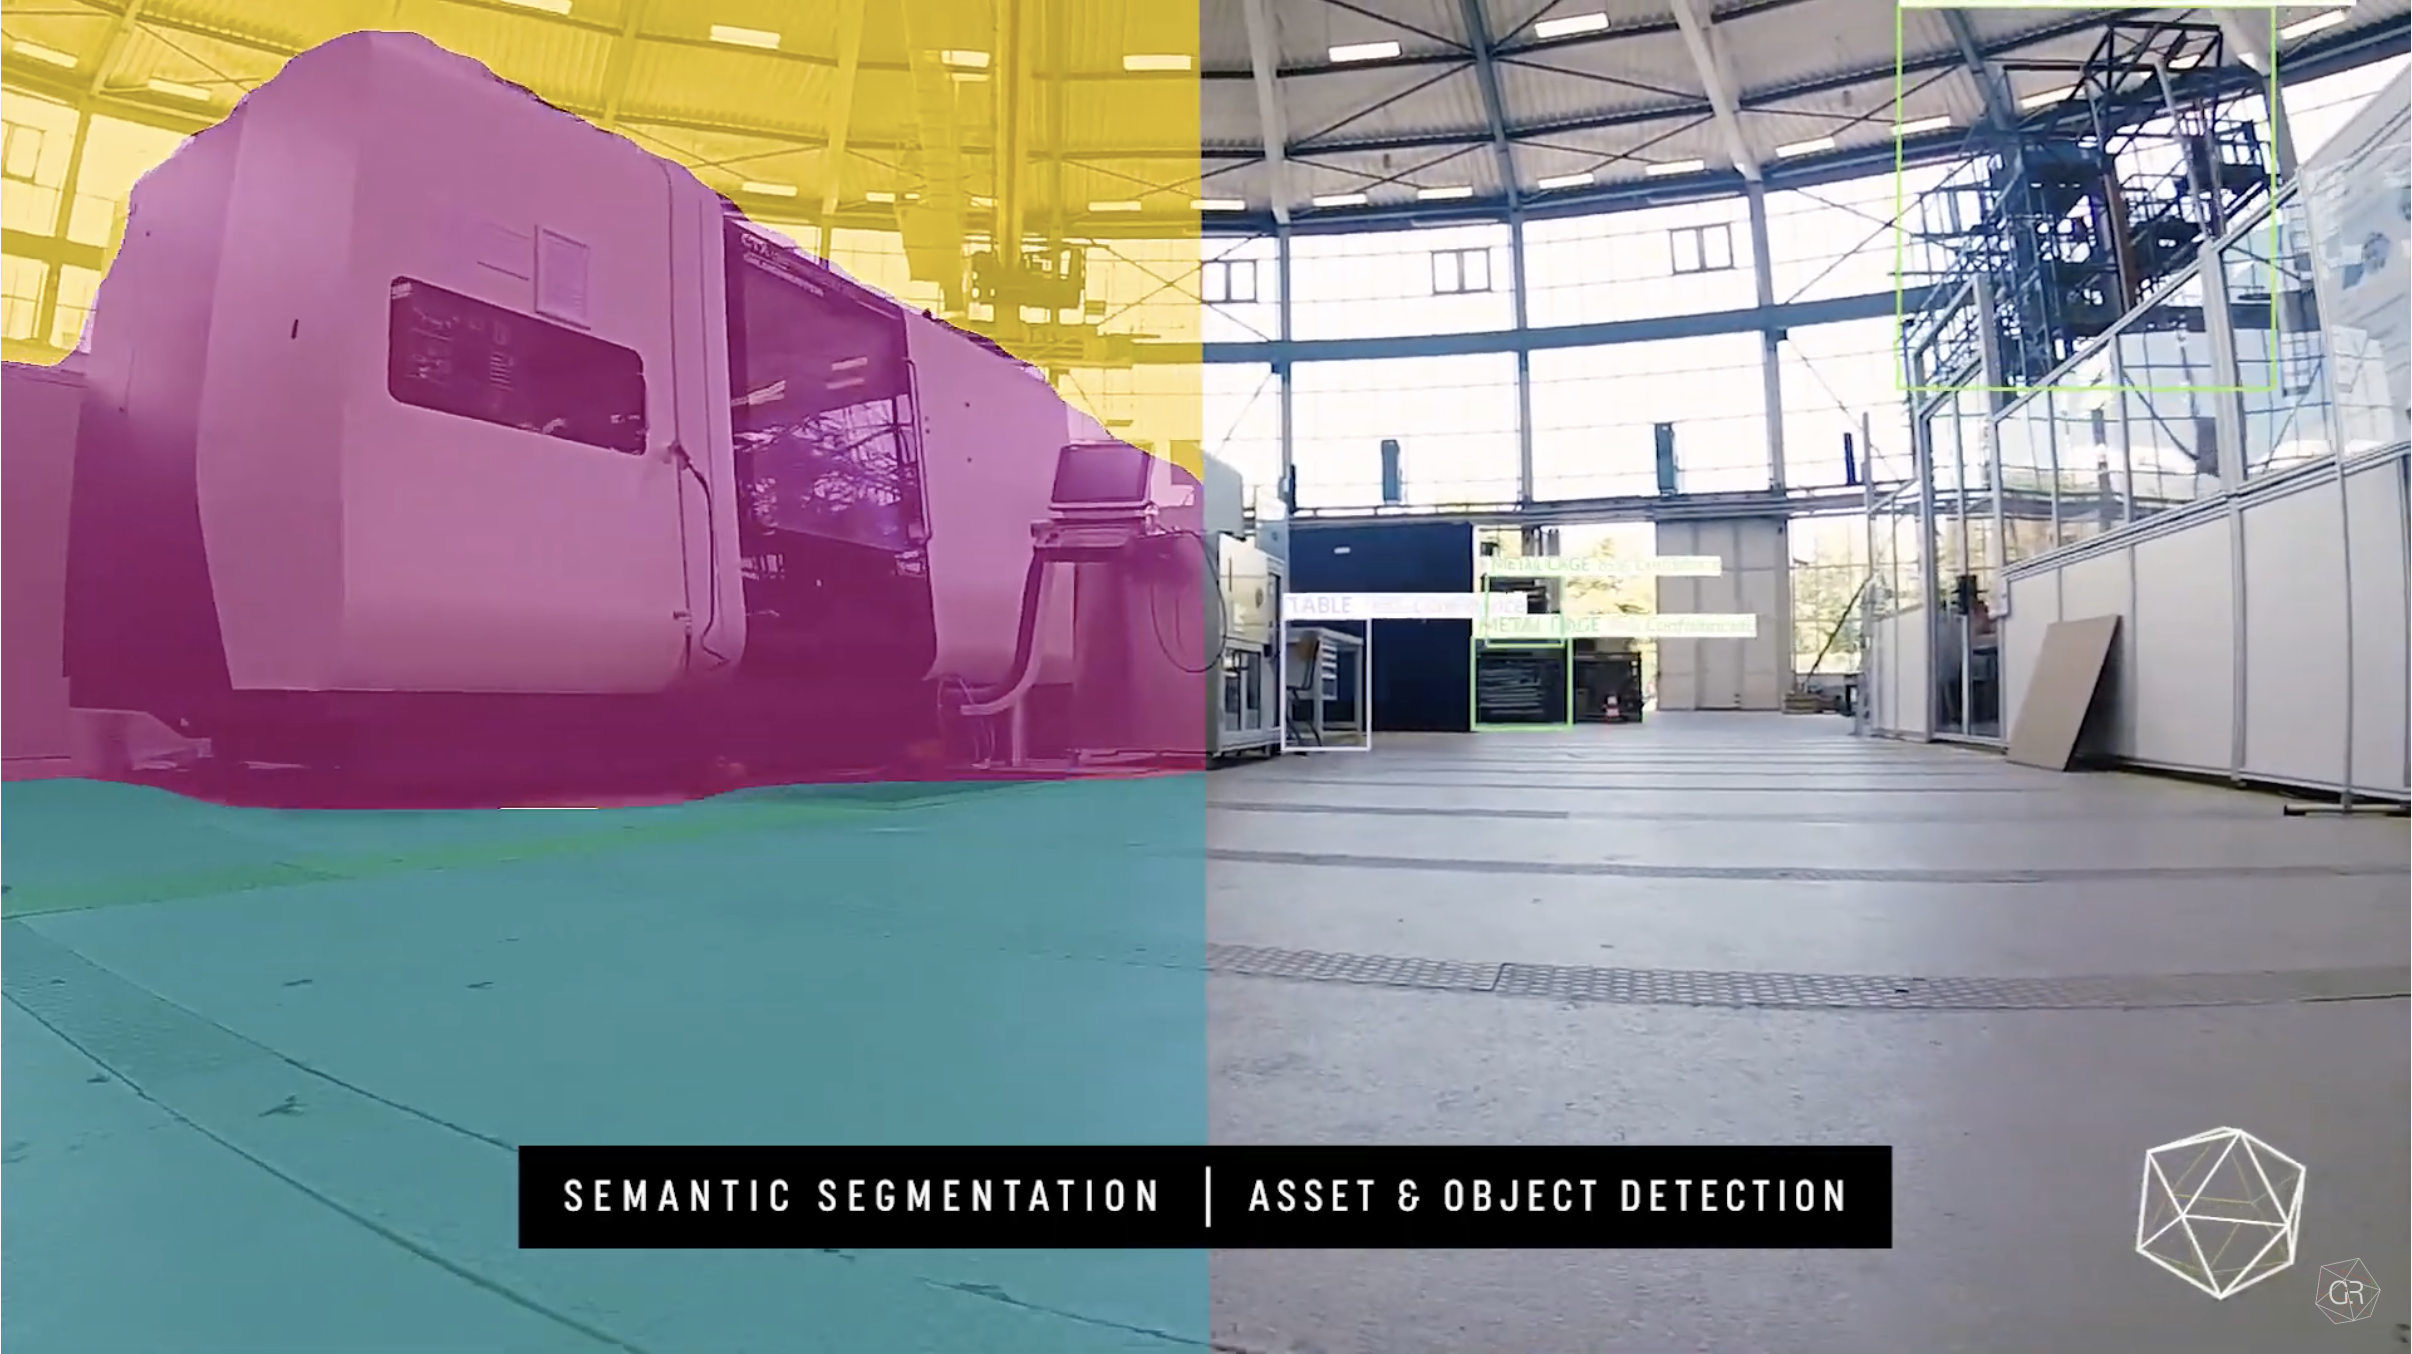
\includegraphics[scale=0.3]{SemanticSegmentation_ObjectDetection.png}
	\caption{Voorbeeld segmentatie + objectdetectie \autocite{Gestalt2019}}
\end{figure}

\subsubsection{Correctheid}
De 2de en meest cruciale factor is de correctheid van het AI-framework voor de verschillende soorten AI-eigenschappen. Het is belangrijk dat het framework betrouwbaar is en dus geen foute oplossing zal terug geven, anders zal dit verkeerd doorgegeven worden aan de visuele kant van de applicatie en zal de route verkeerd worden aangegeven. Om de correctheid van elk AI-framework te testen heeft men opnieuw de diverse AI-eigenschappen onder de loep genomen.

\subsubsection{Correctheid - 1.  Objectdetectie}
Om de objectdetectie te evalueren heeft men geobserveerd of het framework de juiste positie van het gerelateerde object aangeeft , alsook het percentage dat de correctie voorstelt werd in acht gehouden. Dit proces werd 29 keer herhaald, de resultaten werden gebundelend en geëvalueerd. 

\subsubsection{Correctheid - 2. Menssegmentatie}
Bij de evaluatie van de menssegmentatie werd er gekeken of het computer gegenereerde oppervlak overeen kwam met de vorm van de daadwerkelijke persoon. De foute zones werden aangeduid met markeringen om een duidelijk overzicht te krijgen. Deze test werd ook 29 maal herhaald voor elk framework, de resultaten werden telkens naast elkaar gelegd. Om deze eigenschap te evalueren werd een puntensysteem toegepast, elke keer werd een punt uitgedeeld aan het framework die de persoon het beste kon omkaderen. Het framework die na de 29ste test het meeste punten had, werd verkozen als 'winnaar'.

\subsubsection{Correctheid - 3. Luchtsegmentatie}
Luchtsegmentatie werd op dezelfde manier beoordeeld als menssegmentatie. Deze twee segmentaties hebben een zeer gelijkaardige input en output, maar toch is er een groot verschil binnenin het framework. Het algoritme wordt op een andere manier getraind en zo is er toch een mogelijkheid dat deze twee segmentaties voor verschillende resultaten zorgen. Alsook werd deze 29 keer getest, het evaluatieproces werd op dezelfde manier uitgeoefend als bij menssegmentatie.

\subsubsection{Correctheid - 4. Segmentatie binnen gebouwen}
Segmentatie binnen gebouwen is de uitwerking die het meest gerelateerd is met de AI-output die voor deze bachelorproef van belang is. Het biedt namelijk de mogelijkheid om muren van grond te onderscheiden, dit is de hoofdreden waarom men AI in deze wayfinding-uitwerking wilt betrekken. Het is dus belangrijk dat deze AI-uitwerking grondig wordt geëvalueerd.

De evaluatie verliep als volgt, voor beide AI-frameworks werd op identiek dezelfde plaats de test uitgevoerd. Door de relevantie van de technologie was het moeilijk om twee uitgewerkte voorbeelden (TensorFlow Lite en CoreML) te vinden die dezelfde dataset gebruikten. Men heeft deze vergeleken door te kijken hoe goed beide frameworks in hun opzet zijn geslaagd. Dit proces werd alsook 29 keer herhaald, ook deze eigenschap werd op dezelfde manier geëvalueerd zoals lucht en menssegmentatie.
\begin{figure}[H]
	\centering
	\includegraphics[scale=0.3]{BeoordelingsTechnieken.png}
	\caption{Voorbeeld evaluatietechniek segmentatie binnen gebouwen}
\end{figure}

\subsubsection{Toegankelijkheid}
Een tweede belangrijke factor is de toegelankelijkheid van de AI-frameworks voor verschillende platformen. Zo is het belangrijk voor het bedrijf 'In The Pocket' dat ze een oplossing vinden dat schaalbaar is.

\subsubsection{Consistentie}
De derde en laatste factor die men onder de loep zal nemen is consistentie. Dit is een zeer cruciale factor binnen de wayfinding-context, het is belangrijk dat de eindgebruiker zich telkens op een correcte manier naar eindbestemming kan begeven met behulp van de toekomstige app, en niet in bv. 70 \% van de gevallen.

\subsection{Bepalen van optimaal AI-framework}
Het bepalen van welk AI-framework de optimale oplossing biedt werd gemaakt op basis van een overzicht van alle testen. Dit overzicht bevat staafdiagrammen die de resultaten van alle testen in kaart brengt, zo kan men rekening houden met de verschillende eigenschappen die elk framework te bieden heeft.

\chapter{\IfLanguageName{dutch}{Onderzoek}{Research}}
\label{ch:onderzoek}
In dit hoofdstuk zal de effectieve uitwerking van het onderzoek toegelicht worden. In het vorige hoofdstuk werd reeds het 'raamwerk' geschetst, dit hoofdstuk zal hier dus op verder gaan.In dit hoofdstuk zullen volgende zaken toegelicht worden:

\begin{itemize}
	\item Het bestuderen van de verschillende frameworks
	\item De AI-eigenschappen van elk framework valideren naargelang een vooropgestelde trainingset
	\item De resultaten bespreken voor elke AI-eigenschap
\end{itemize}

\section{De beproeving van de frameworks}
In deze sectie zullen de effectieve tests worden uitgevoerd, men zal steeds de resultaten van elk algoritme bespreken.

\subsection{Objectdetectie}

Zoals men eerder al heeft vermeld is objectdetectie een belangrijke factor binnen de wayfinding-context, men zal namelijk moeten weten waar elk object binnen een bepaalde kamer zich bevindt. Om dit op een goede manier te kunnen testen heeft men vijf verschillende objecten genomen en getest of men verschillende waarnemingen kon constateren. Om de resultaten te kunnen meten heeft men gebruik gemaakt van twee verschillende applicaties, 'Fritz AI Studio' en 'TFL Detect', beide applicaties werden uitgevoerd op een iPhone 11 (camera: 12MP). Beide frameworks maakten immers gebruik van de COCO dataset.


\subsubsection{Tests}
	\begin{figure}[H]
		\centering
		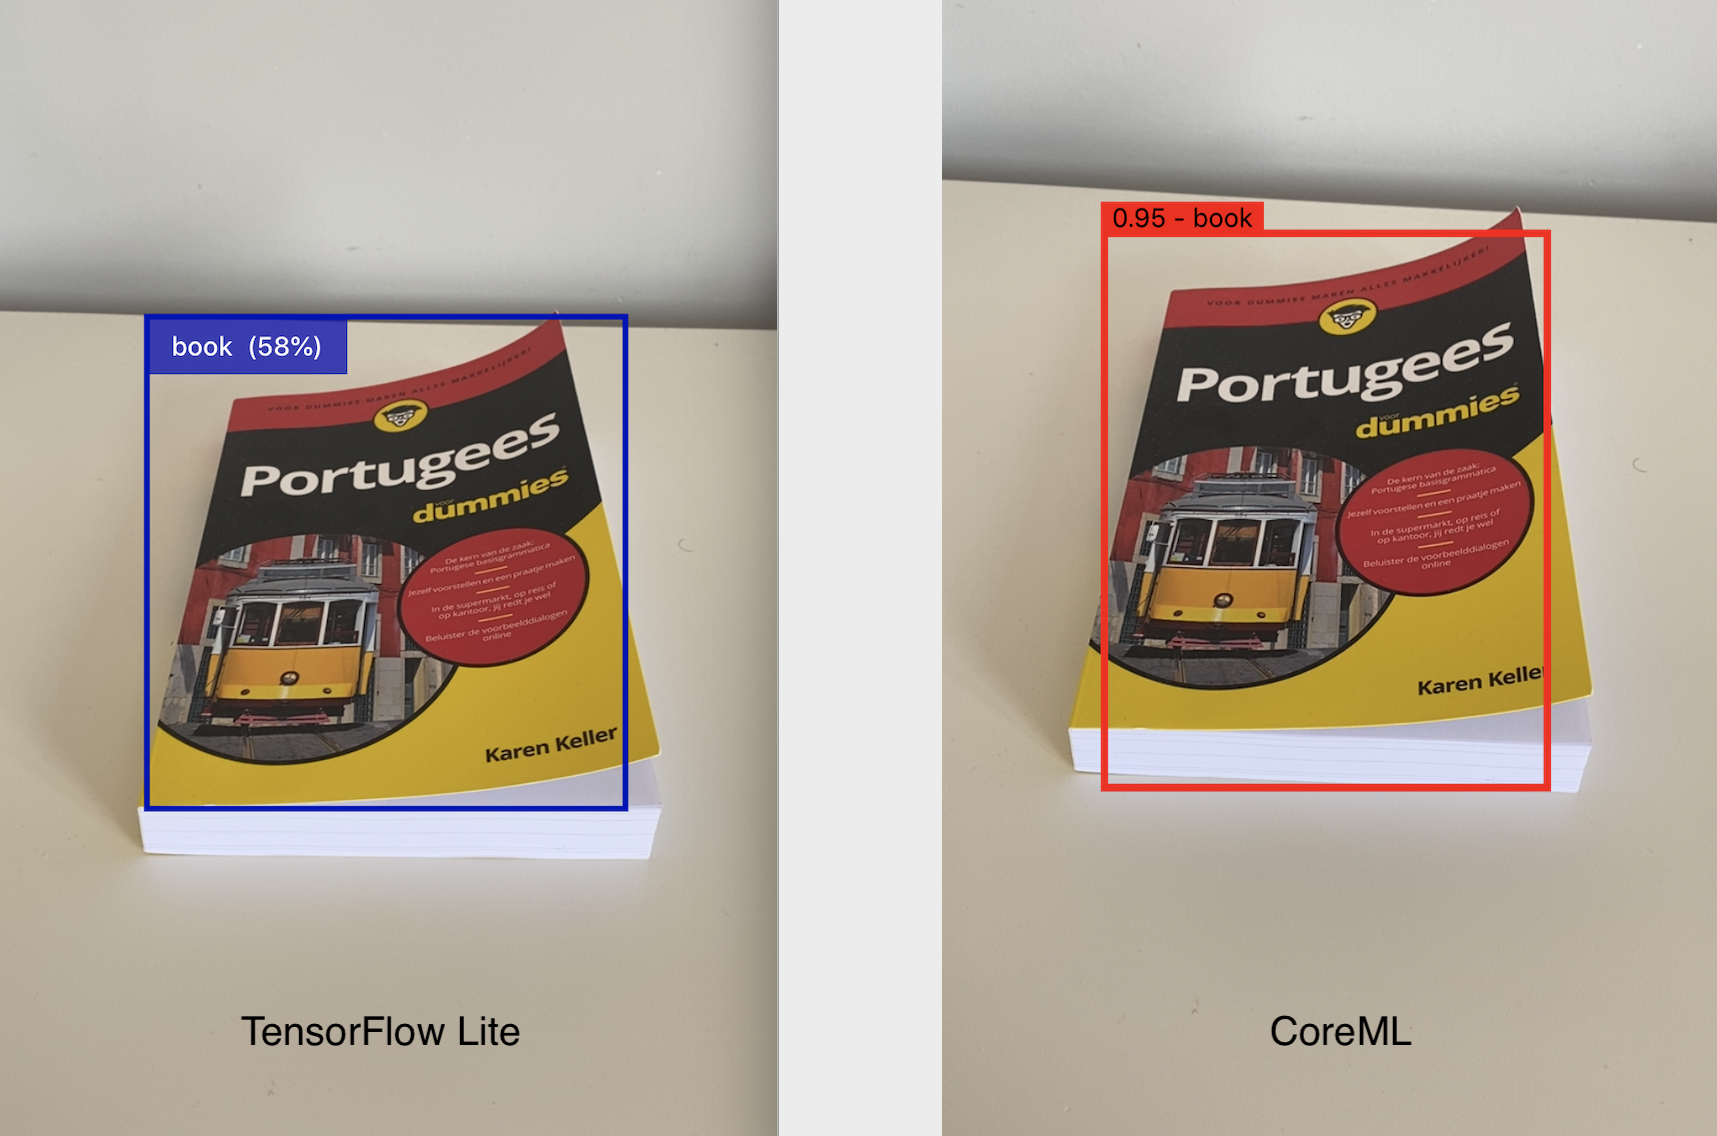
\includegraphics[scale=0.3]{ObjectDetection_Book.png}
		\caption{Test met boek, TensorFlow Lite (58\%) \& CoreML (95 \%)}
	\end{figure}
In de eerste objectdetectie-test kan men reeds waarnemen dat het boek beter wordt gedetecteerd door het CoreML-framework. Ten eerste wordt het boek nauwkeuriger aangeduid door de rechthoek, en ten tweede is het percentage veel beter. Het percentage dat de zekerheid aanduidt is namelijk 95 \% bij CoreML en 58 \% bij TensorFlow Lite. Dit redeneringsproces heeft men 29 keer herhaald.

\begin{figure}[H]
	\centering
	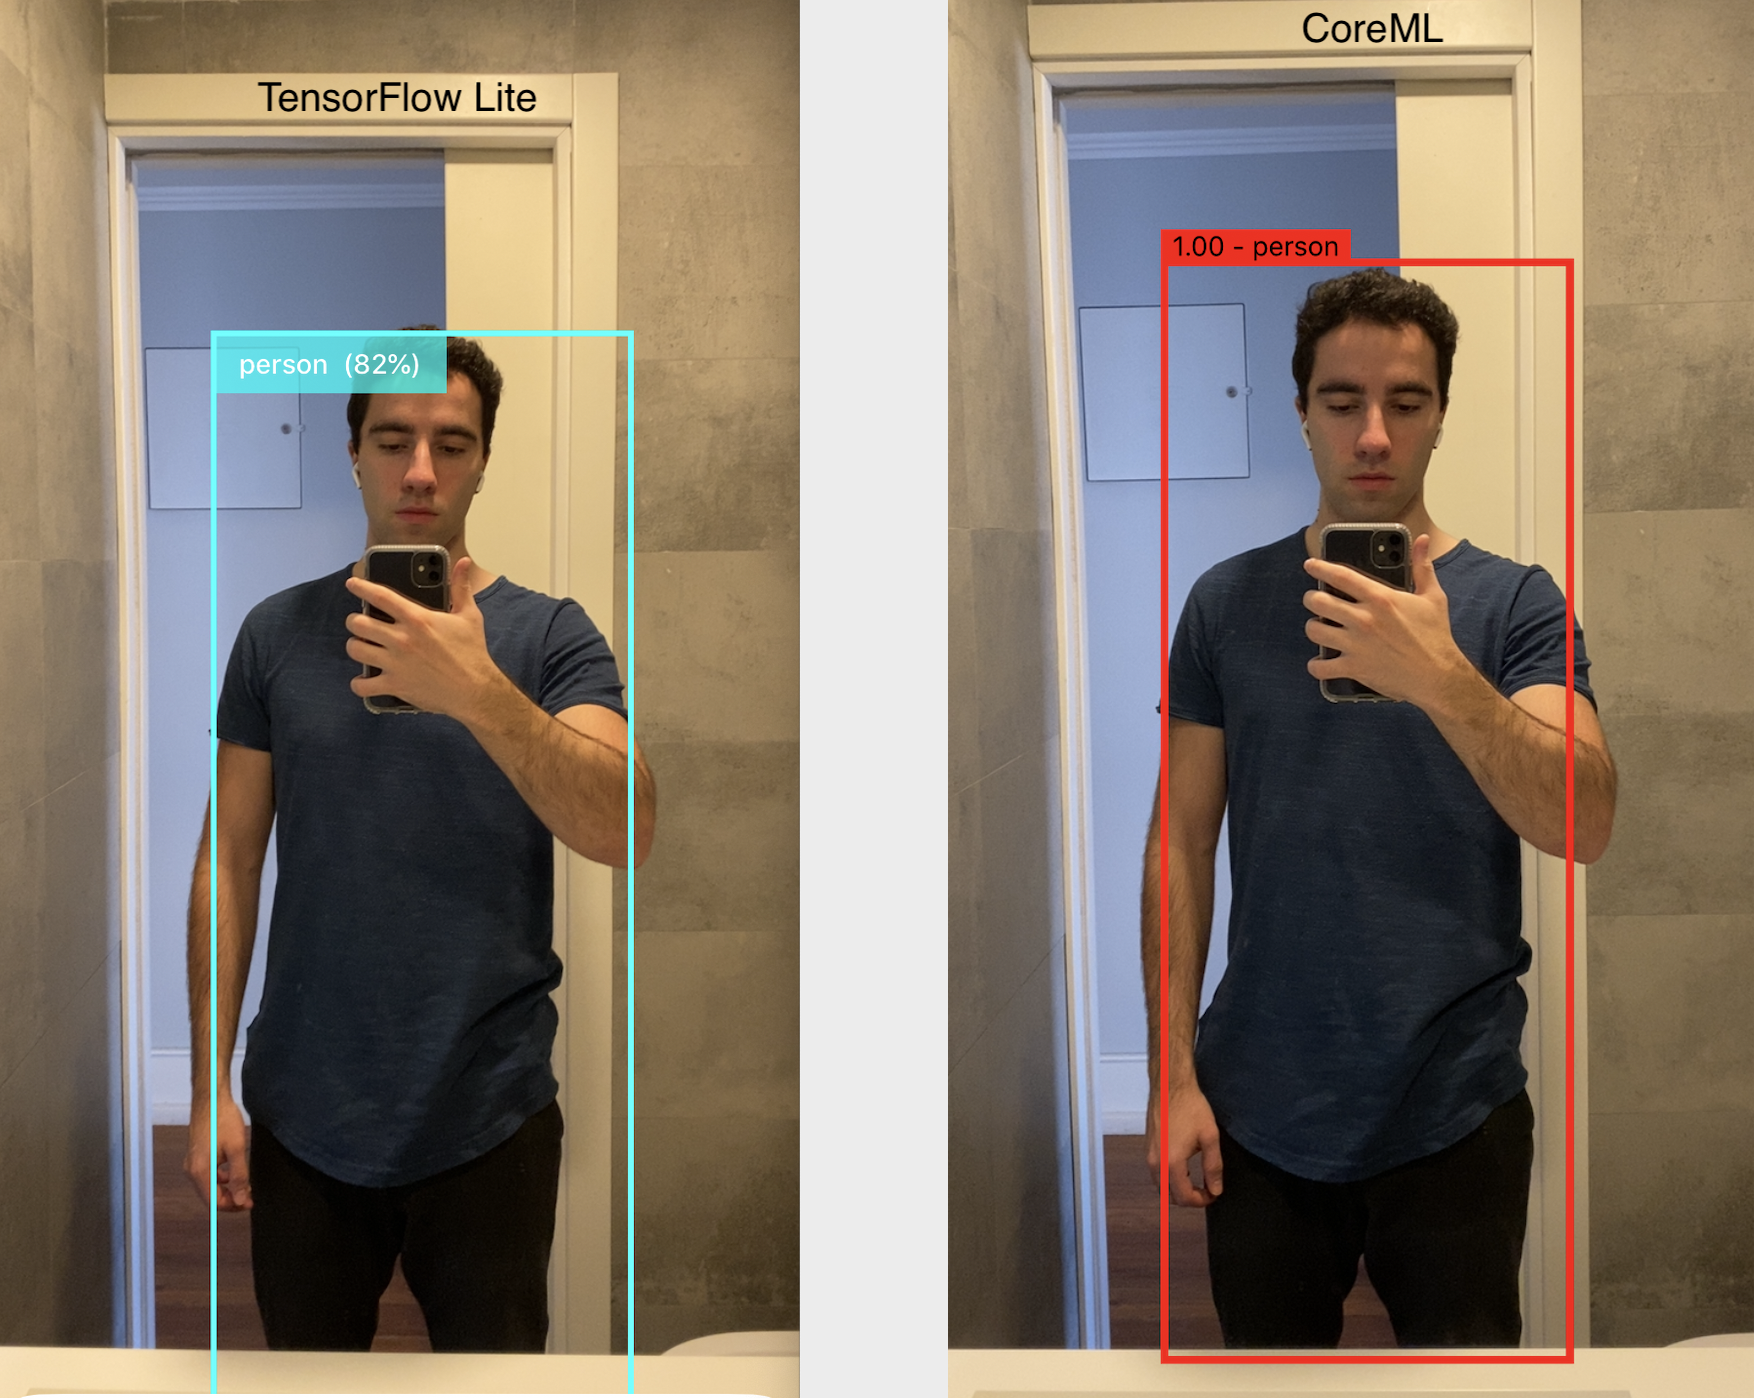
\includegraphics[scale=0.3]{ObjectDetection_Person.png}
	\caption{Test met persoon, TensorFlow Lite (82\%) \& CoreML (100 \%)}
\end{figure}
De tweede test toont nogmaals aan dat CoreML beter scoort. De persoon wordt veel exacter aangeduid met behulp van het vierkant. Het correctheidspercentage is nogmaals beter bij het CoreML-framework, men kan zelfs opmerken dat dit framework met 100\% kan zeggen dat het object een persoon is, dit resultaat is zeer opmerkelijk. Om te testen of de AI-frameworks consistent acteren heeft men dit redeneringsproces 29 maal herhaald.

\begin{figure}[H]
	\centering
	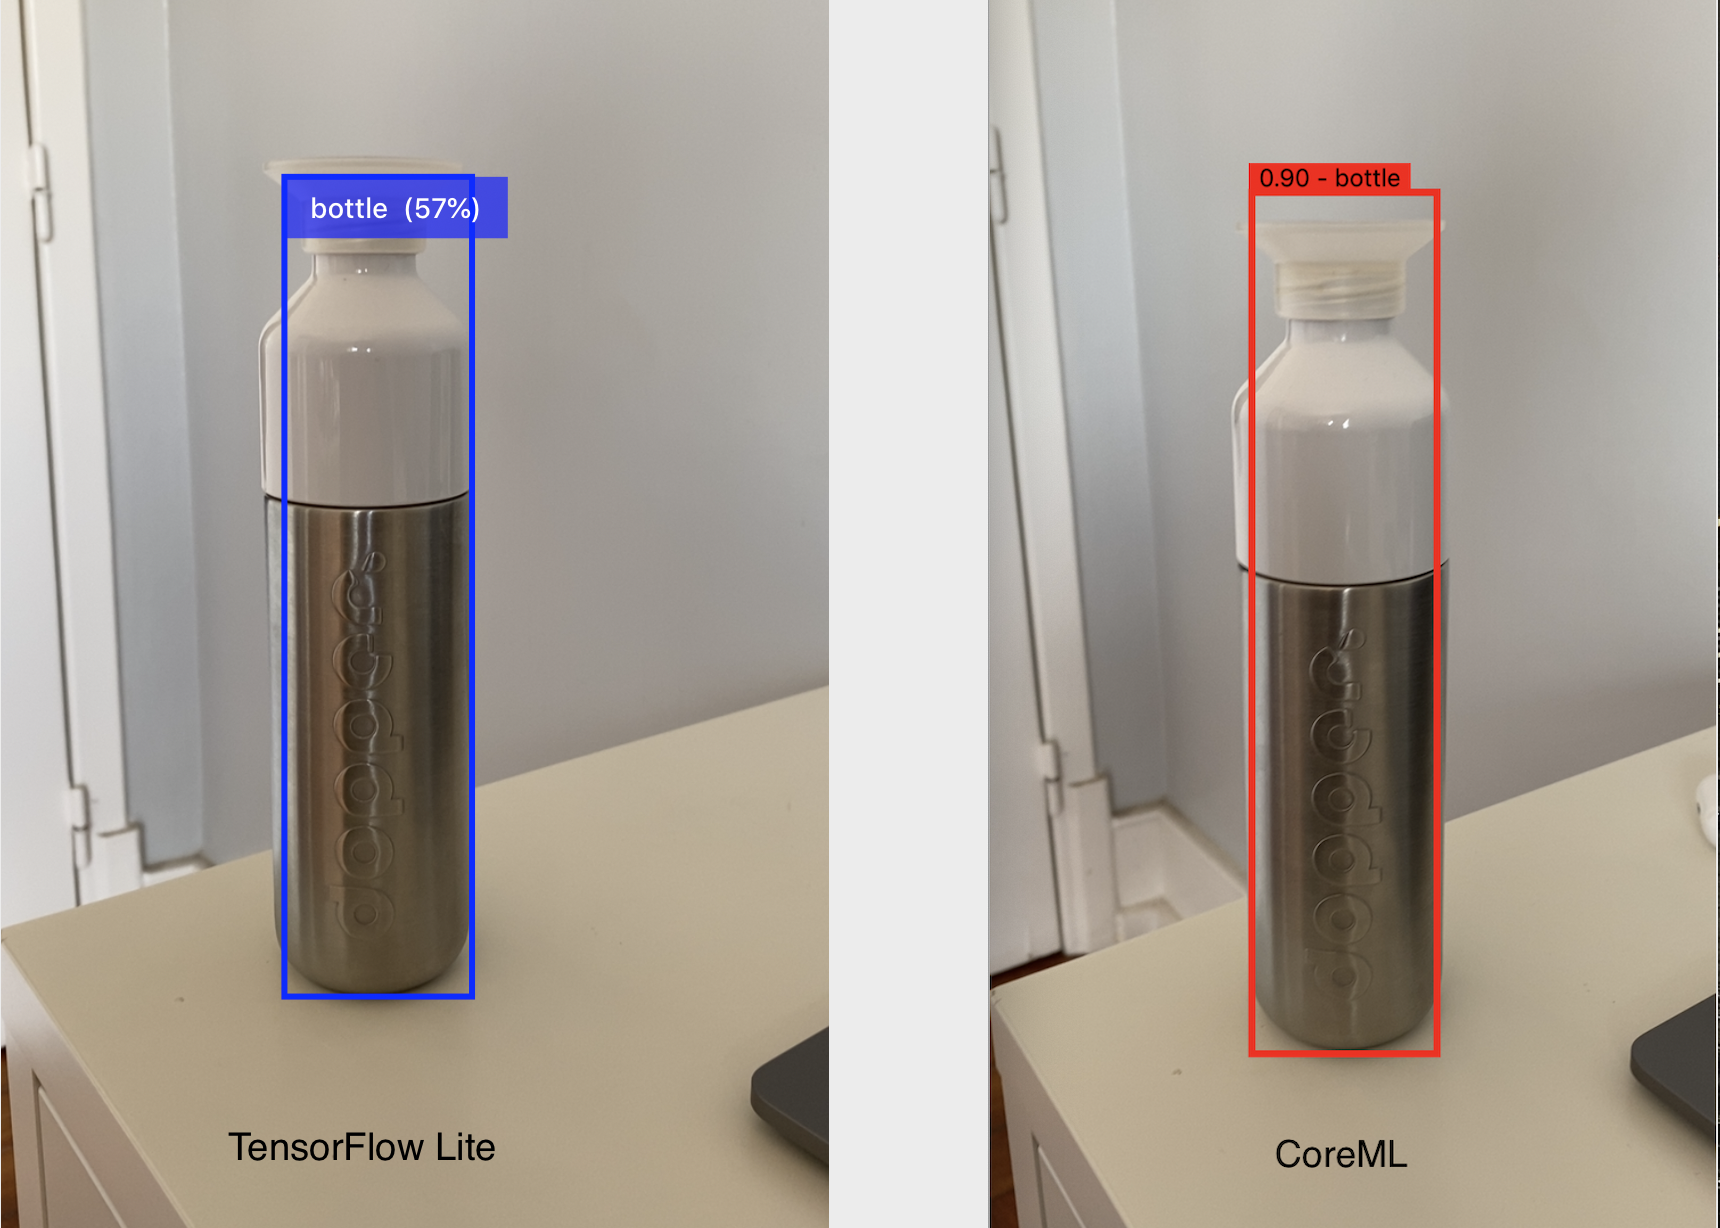
\includegraphics[scale=0.35]{ObjectDetection_Bottle.png}
	\caption{Test met waterfles, TensorFlow Lite (57\%) \& CoreML (90 \%)}
\end{figure}
Men kan opnieuw besluiten dat het framework van Apple een betere zaak doet om de waterfles te herkennen. Opnieuw kan men een significant correctheidsverschil opmerken tussen beide frameworks. CoreML kan in dit geval men bijna 30 \% meer zekerheid zeggen dat het vertoonde object een fles is. Ook voor dit object werd deze test 29 maal herhaald.
\begin{figure}[H]
	\centering
	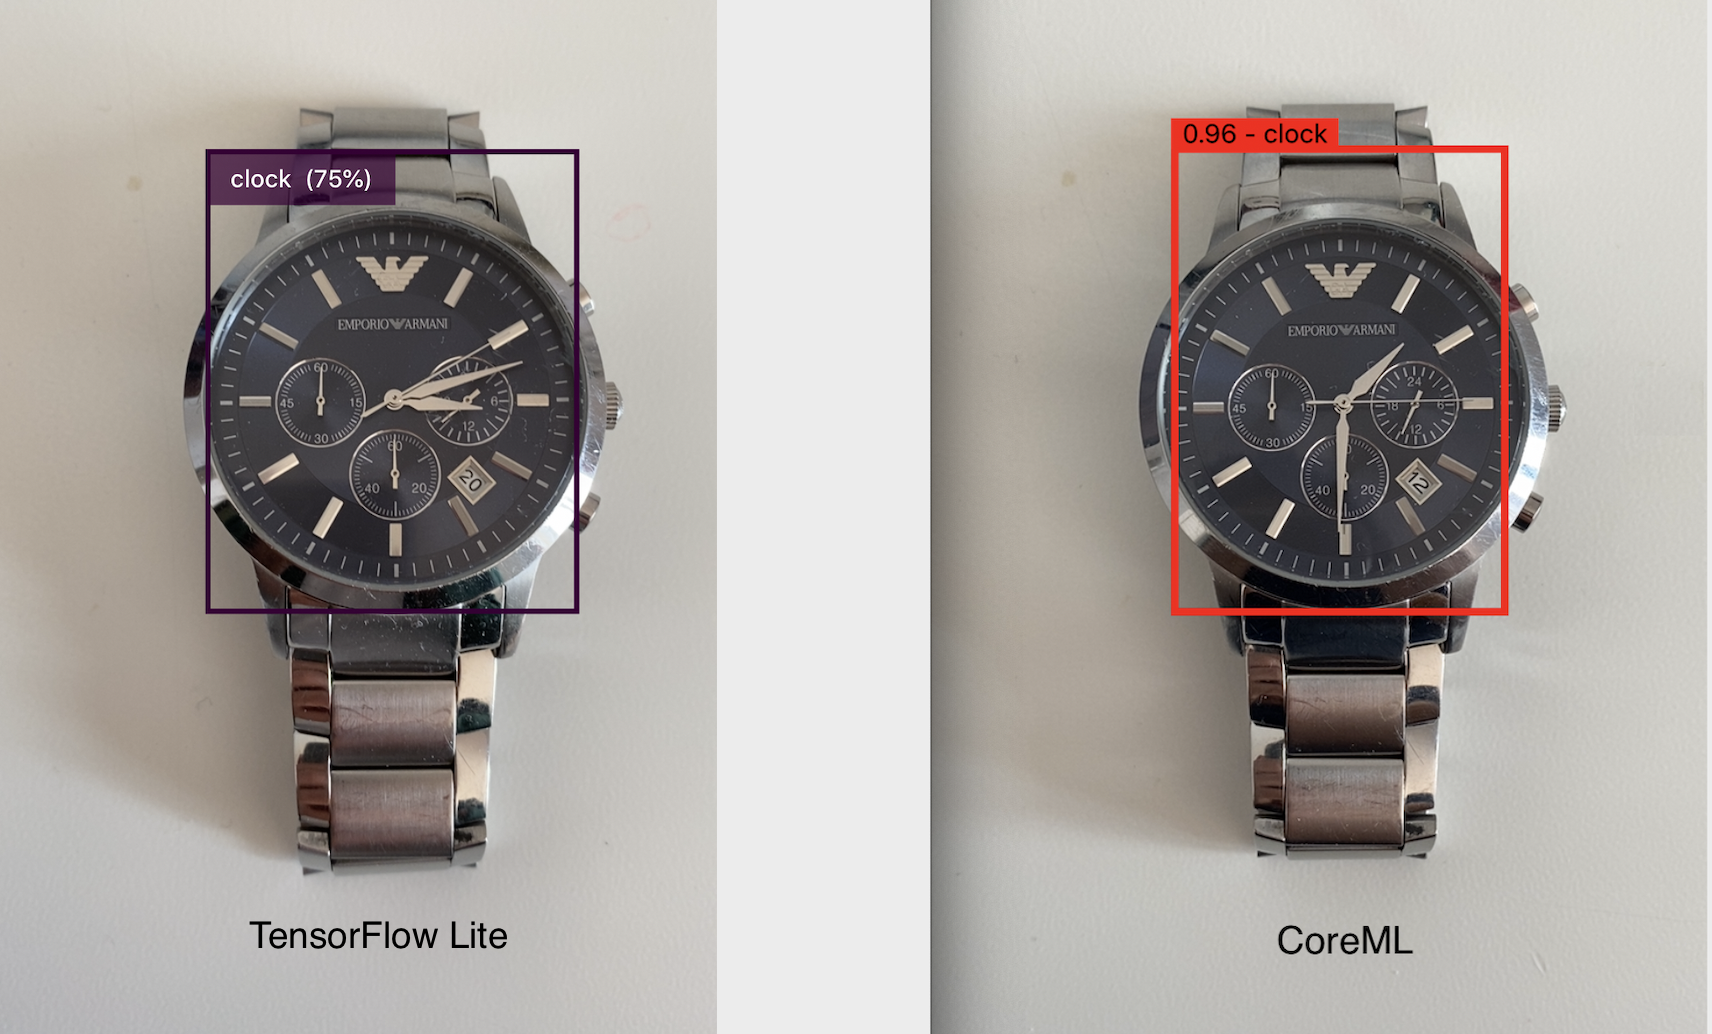
\includegraphics[scale=0.38]{ObjectDetection_Clock.png}
	\caption{Test met horloge, TensorFlow Lite (75 \%) \& CoreML (96 \%)}
\end{figure}
Andermaal kan men waarnemen dat het CoreML-framework betere resultaten levert als TensorFlow Lite, men kan in dit geval wel opmerken dat de detectie a.d.h.v het vierkant nauwkeuriger werd uitgevoerd door het TensorFlow Lite-framework. Opnieuw kan men een nauwkeurigheidsverschil opmerken van meer dan 20 \%. Dit redeneringsproces werd ook 29 maal herhaald om te achterhalen of de resultaten wel consistent zijn.

\begin{figure}[H]
	\centering
	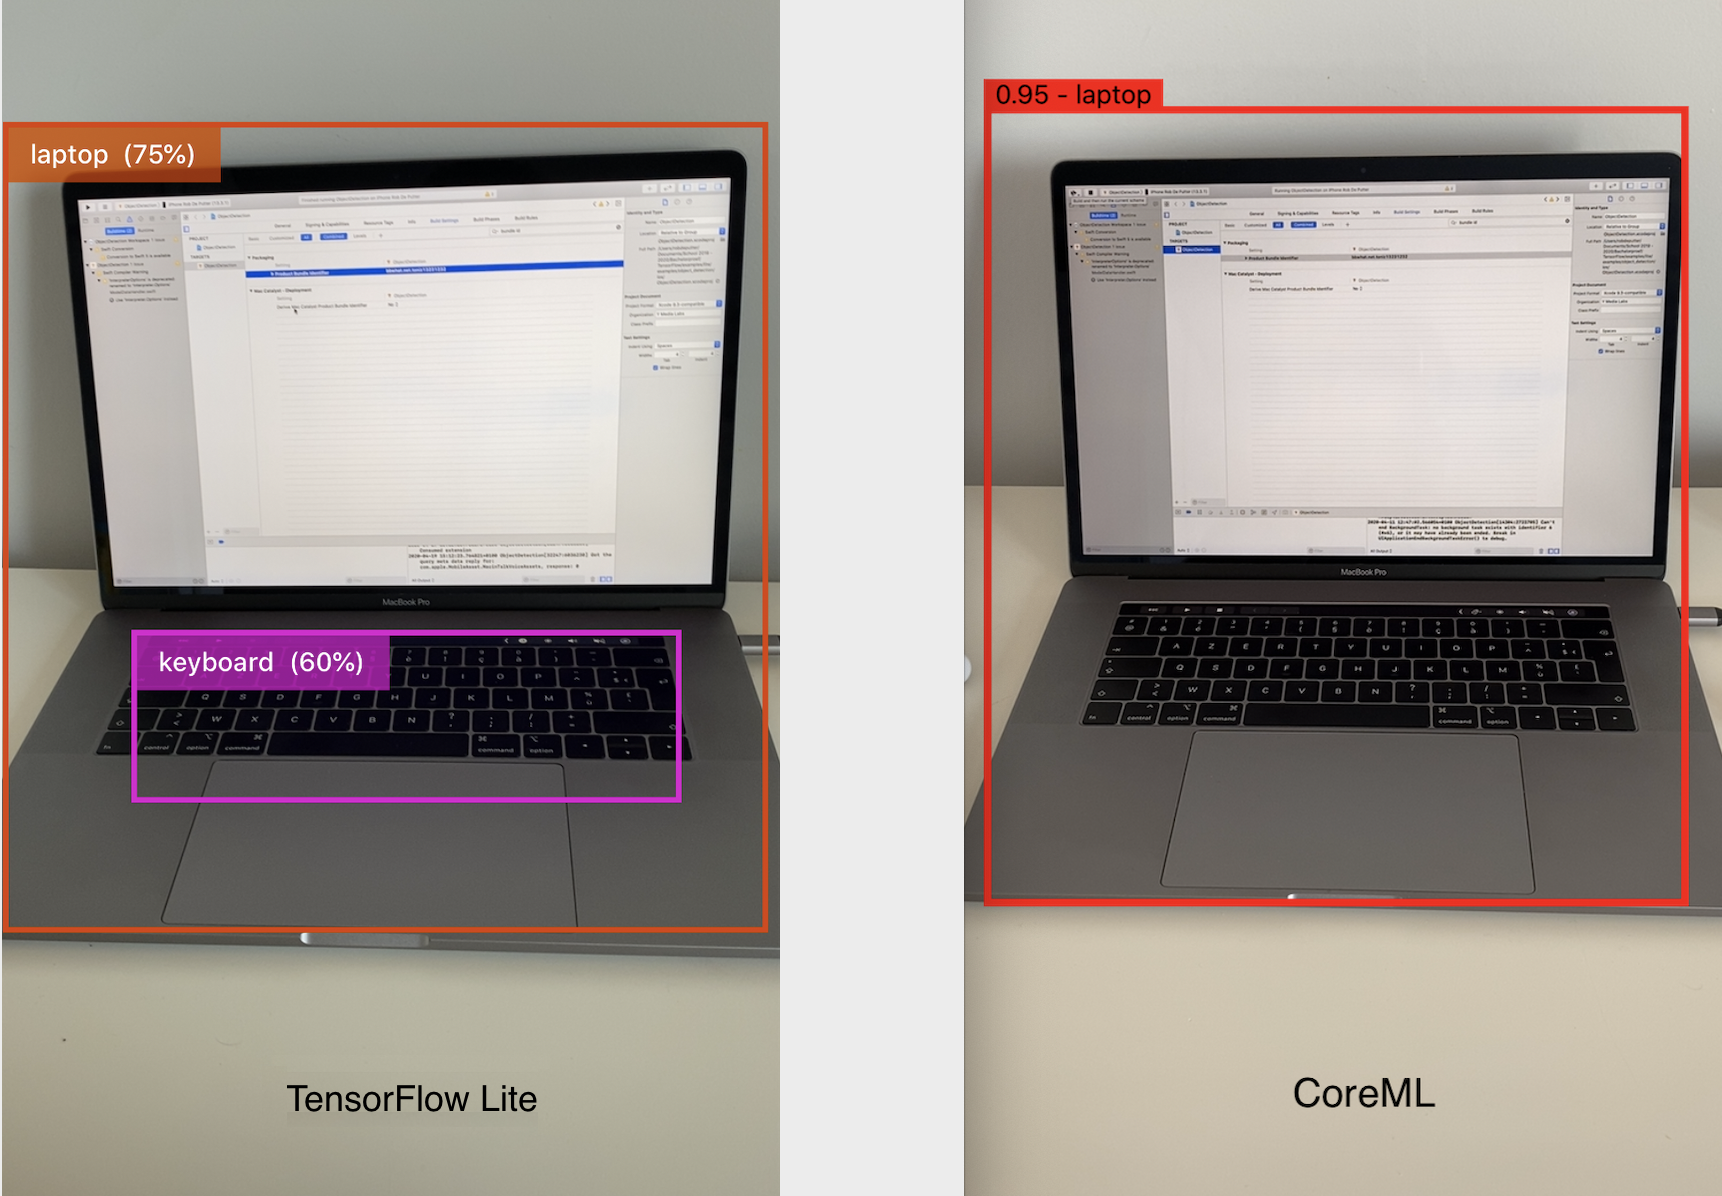
\includegraphics[scale=0.38]{ObjectDetection_Laptop.png}
	\caption{Test met laptop, TensorFlow Lite (75 \%) \& CoreML (95 \%)}
\end{figure}
De laatste test verschilt van de anderen, men kan namelijk bemerken dat TensorFlow Lite het toestenbord kan bespeuren, terwijl CoreML niet in staat is om dit te doen. De nauwkeurigheid kent wel lagere cijfers, opnieuw is er een verschil van 20 \% op vlak van accuraatheid. Alsook de laptoptest werd 29 maar herhaald. 
	

\subsection{Menssegmentatie}
De tweede AI-eigenschap die men getest heeft is menssegmentatie, in deze eigenschap zal men de volledige foto gaan onderzoeken of er zich mensen in begeven. Indien er zich mensen in het beeld bevinden zal het algoritme deze aanduiden door een bepaald kleuroppervlak over deze objecten te plaatsen. De resultaten werden bekomen door gebruik te maken van de 'Fritz AI Studio' applicatie op twee verschillende apparaten, namelijk een iPhone 11 (camera: 12MP) (iOS) en een Huawei P20 Lite (camera: 16MP) (Android). In de documentatie van de 'Fritz AI Studio' applicatie kan men opmerken dat de Android-variant gebruik maakt van TensorFlow Lite en de iOS-variant CoreML utiliseert. Deze beide frameworks gebruiken hetzelfde voorgetrainde model, dit werd samengesteld door Fritz AI.

\newpage
\subsubsection{Test}

\begin{figure}[H]
	\centering
	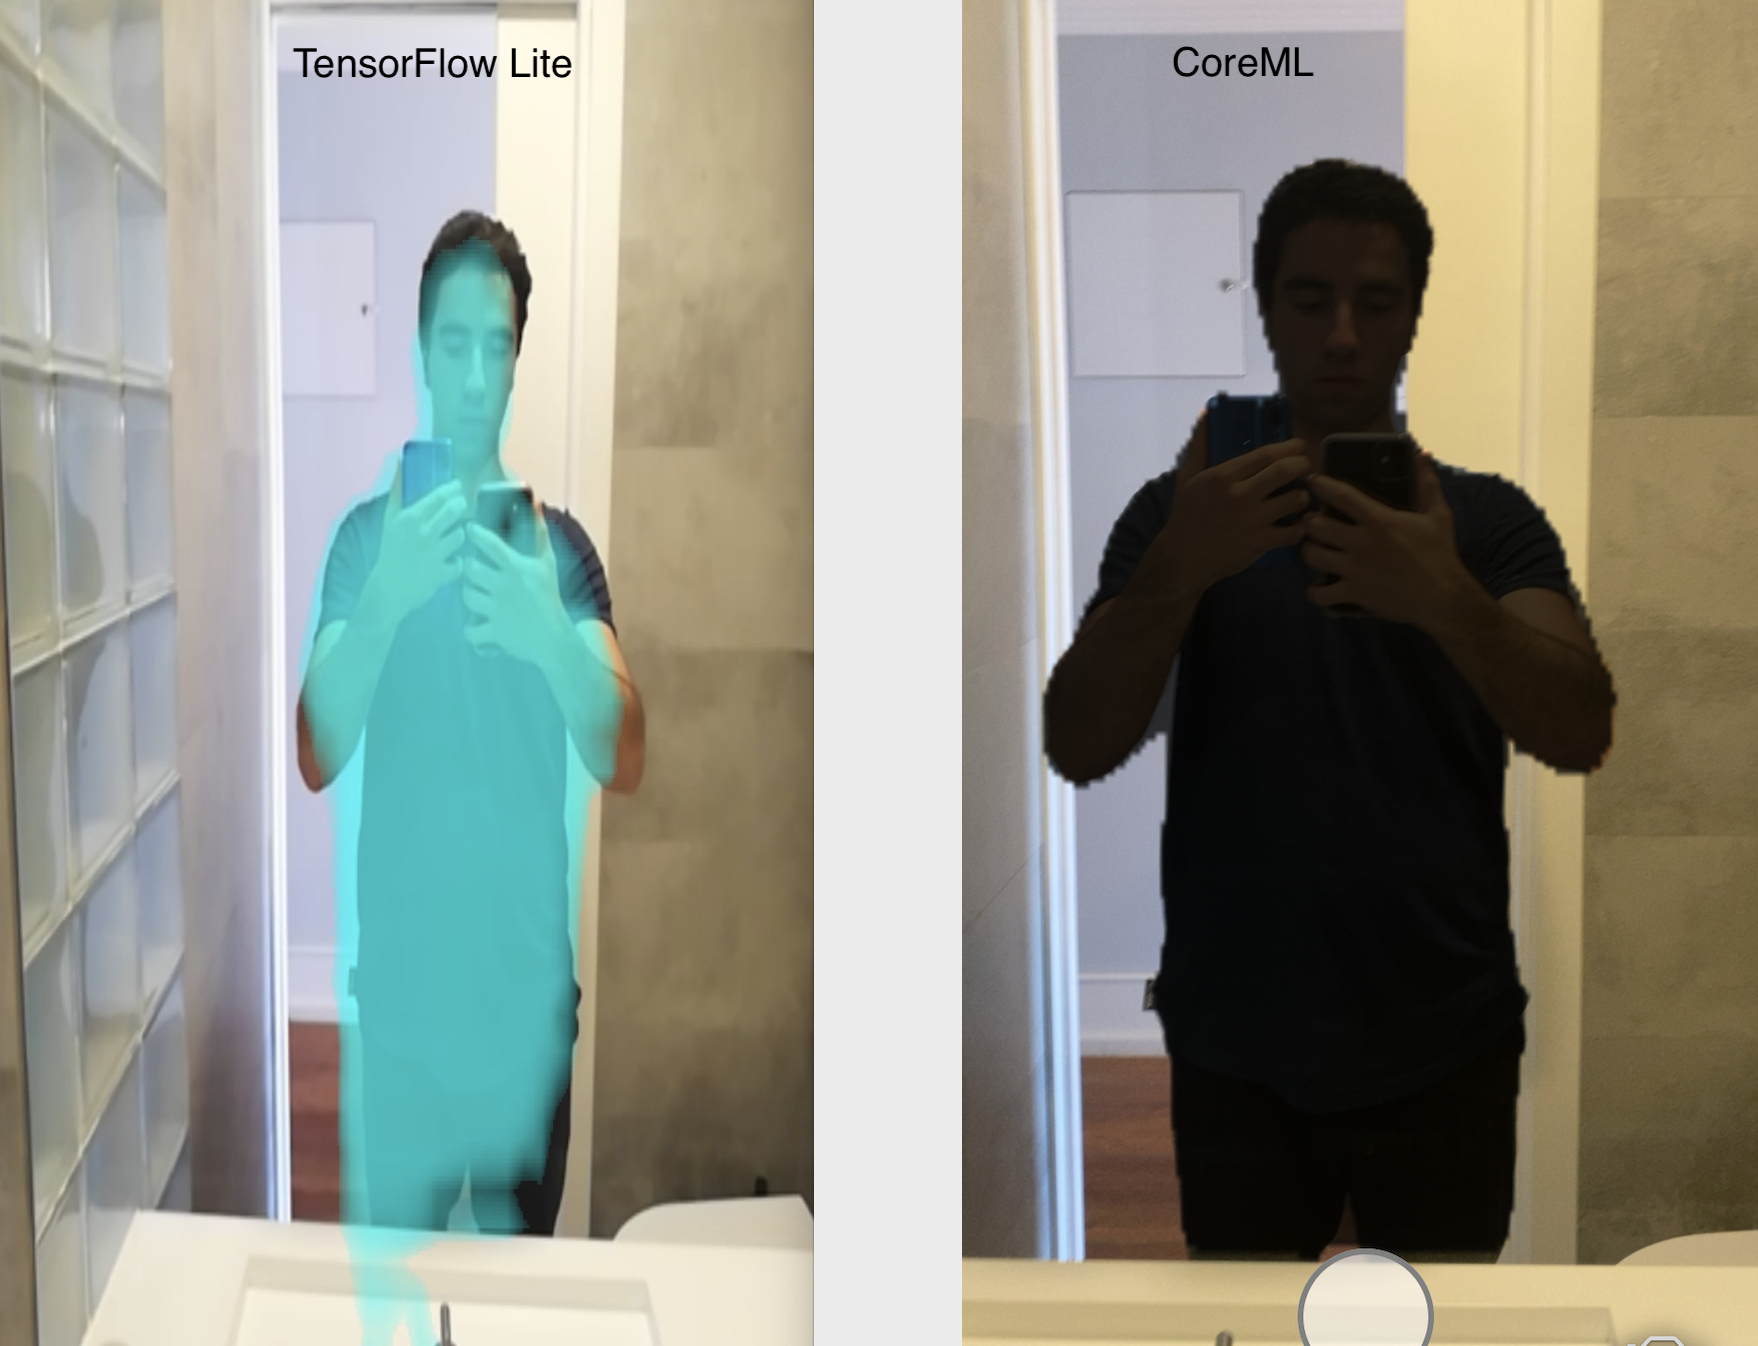
\includegraphics[scale=0.4]{PeopleSegmentation.png}
	\caption{Test menssegmentatie, zonder foutaanduiding}
\end{figure}
Uit de resultaten van deze test kan men opnieuw aanschouwen dat het CoreML-framework een veel betere uitslag levert dan TensorFlow Lite. Ondanks dezelfde dataset slaagt CoreML er in deze test toch in om de persoon in de afbeelding bijna 100 \% correct aan te duiden, de uitkomst van het andere framework is niet nauwkeurig en kent zelfs grove fouten. Men kan in deze test concluderen dat het CoreML-framework veel nauwkeuriger is. In de onderstaande afbeelding kan men de foute zones waarnemen, de rode vlaktes tonen aan waar de persoon niet werd gedetecteerd, maar wel was. Het gele gebied duidt de zones aan waar de persoon werd gedetecteerd, maar niet was. Dit visueel redeneringsproces werd 29 maal herhaald, telkens kreeg het framework met de minste foute zones een punt, het framework dat na de 29ste test het meeste punt haalde zou dit deelexperiment 'winnen'.

 De link tussen menssegmentatie en de wayfinding-context kan misschien ver te zoeken zijn, maar deze test zegt wel degelijk meer over de precisie van het AI-framework. Alsook is het mogelijk dat een groep mensen de weg kan versperren, in dit geval is het belangrijk dat deze groep wordt gedetecteerd door het algoritme, een zekere mensherkenning en detectie is dus zeker van belang.

\begin{figure}[H]
	\centering
	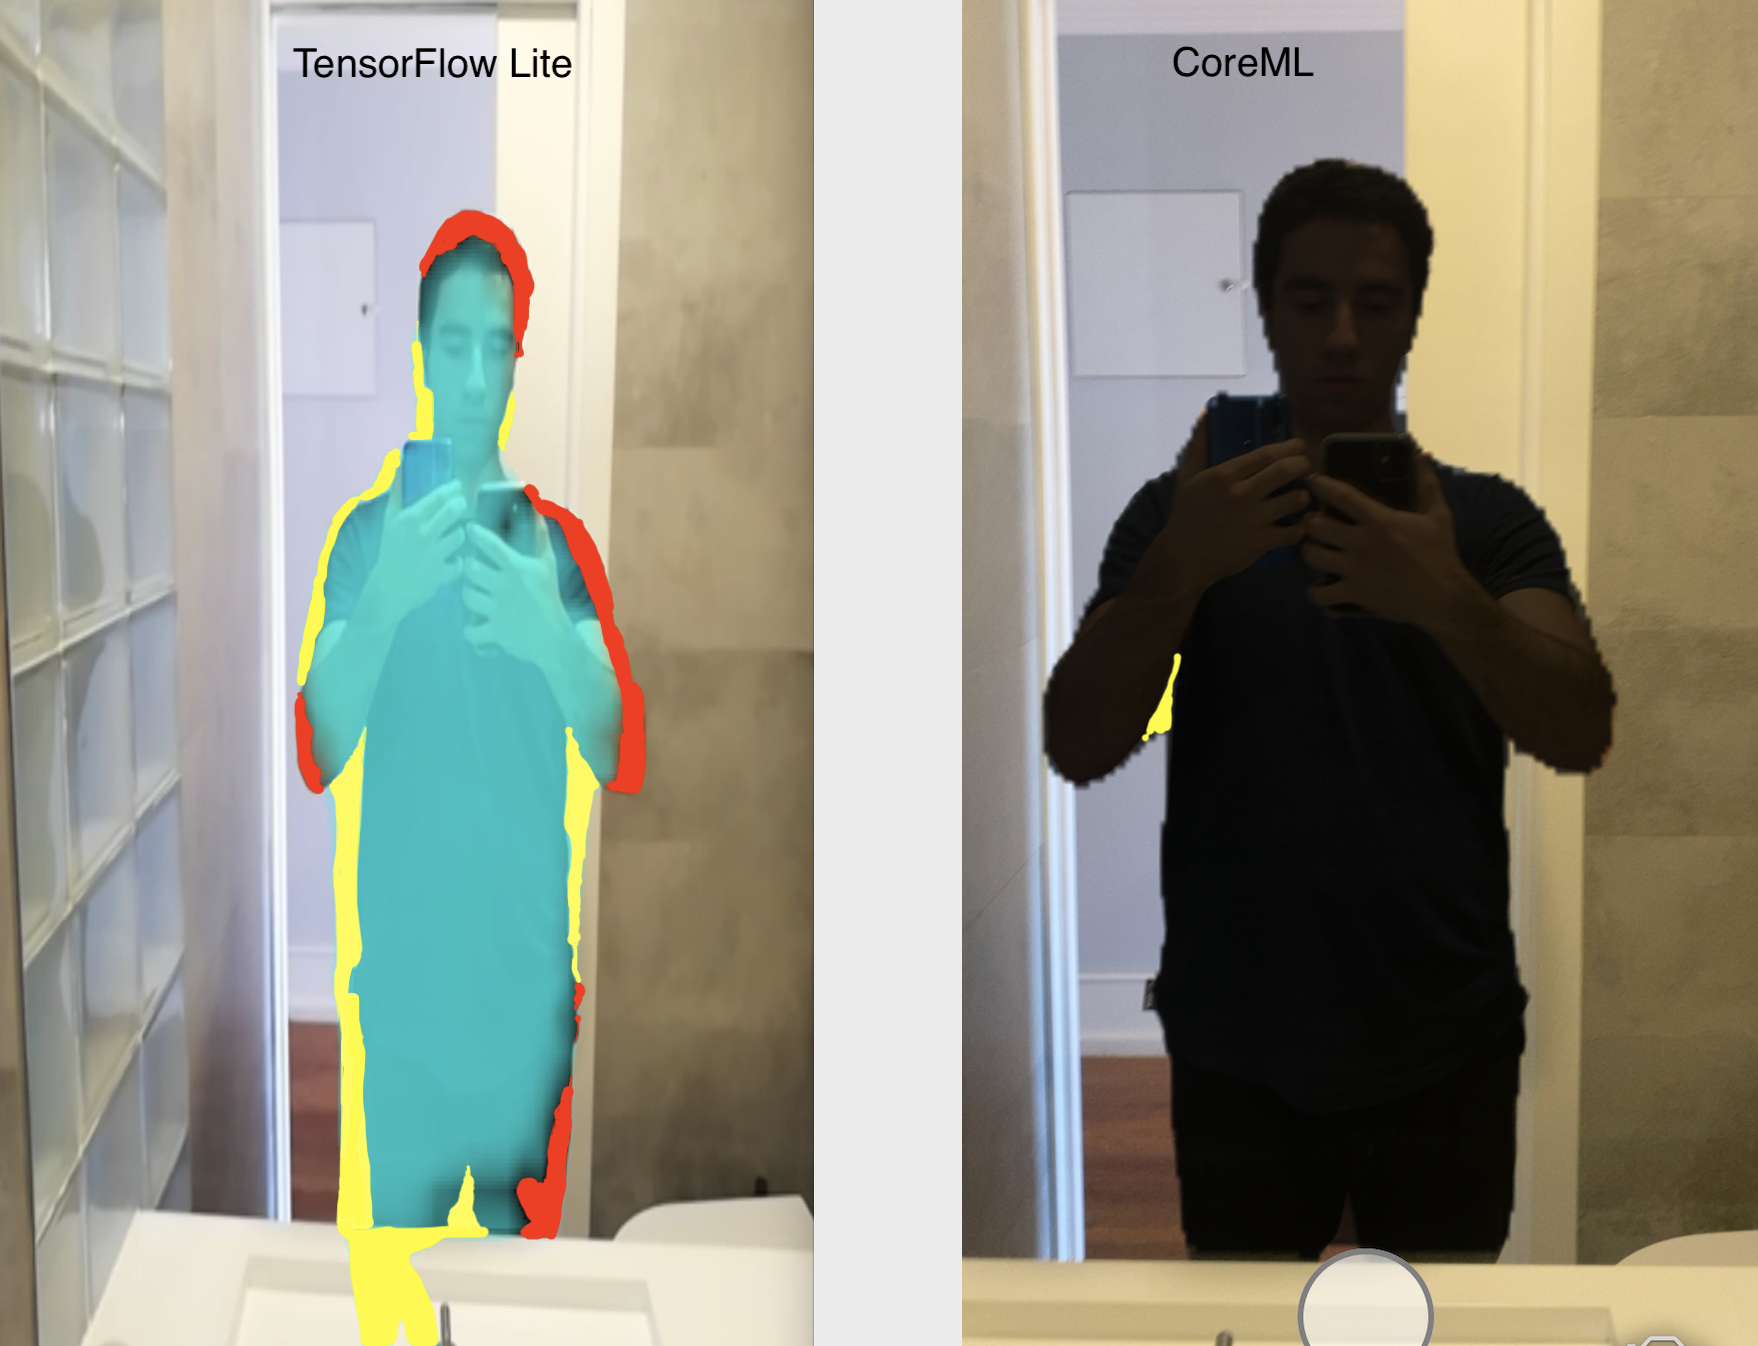
\includegraphics[scale=0.45]{PeopleSegmentation_MetFoutAanduiding.png}
	\caption{Test menssegmentatie, met foutaanduiding}
\end{figure}

\subsection{Luchtsegmentatie}
Om de AI-frameworks andermaal op nauwkeurig -en correctheid te testen, heeft men ervoor gekozen om ook luchtsegmentatie te observeren. Luchtsegmentatie zal net zoals menssegmentatie gekleurde vlekken plaatsen over de regio's waar men lucht detecteert. Alsook kan men bij deze AI-eigenschap denken dat dit geen direct verband heeft met de wayfinding context, maar toch geeft dit een extra beeld over hoe correct en nauwkeurig het AI-algoritme de verschillende vlakken kan onderscheiden. Zoals men eerder al aangaf in de methodologie zal men de foute zones aanduiden, het algoritme met het merendeel aan foute zones zal mogelijks niet worden geselecteerd als 'eindwinnaar'. Om deze test te kunnen uitvoeren werd de applicatie 'AI Fritz Studio' gebruikt, ook in dit onderzoek heeft men de applicatie beproeft op twee verschillende apparaten. Het CoreML-framework werd getest op een iPhone 11 (camera: 12MP), TensorFlow Lite werd uitgevoerd op een Huawei P20 Lite (camera: 16MP) (Android). Beide frameworks werden getrained met een dataset die werd opgesteld door Fritz AI.

\newpage
\subsubsection{Test}
\begin{figure}[H]
	\centering
	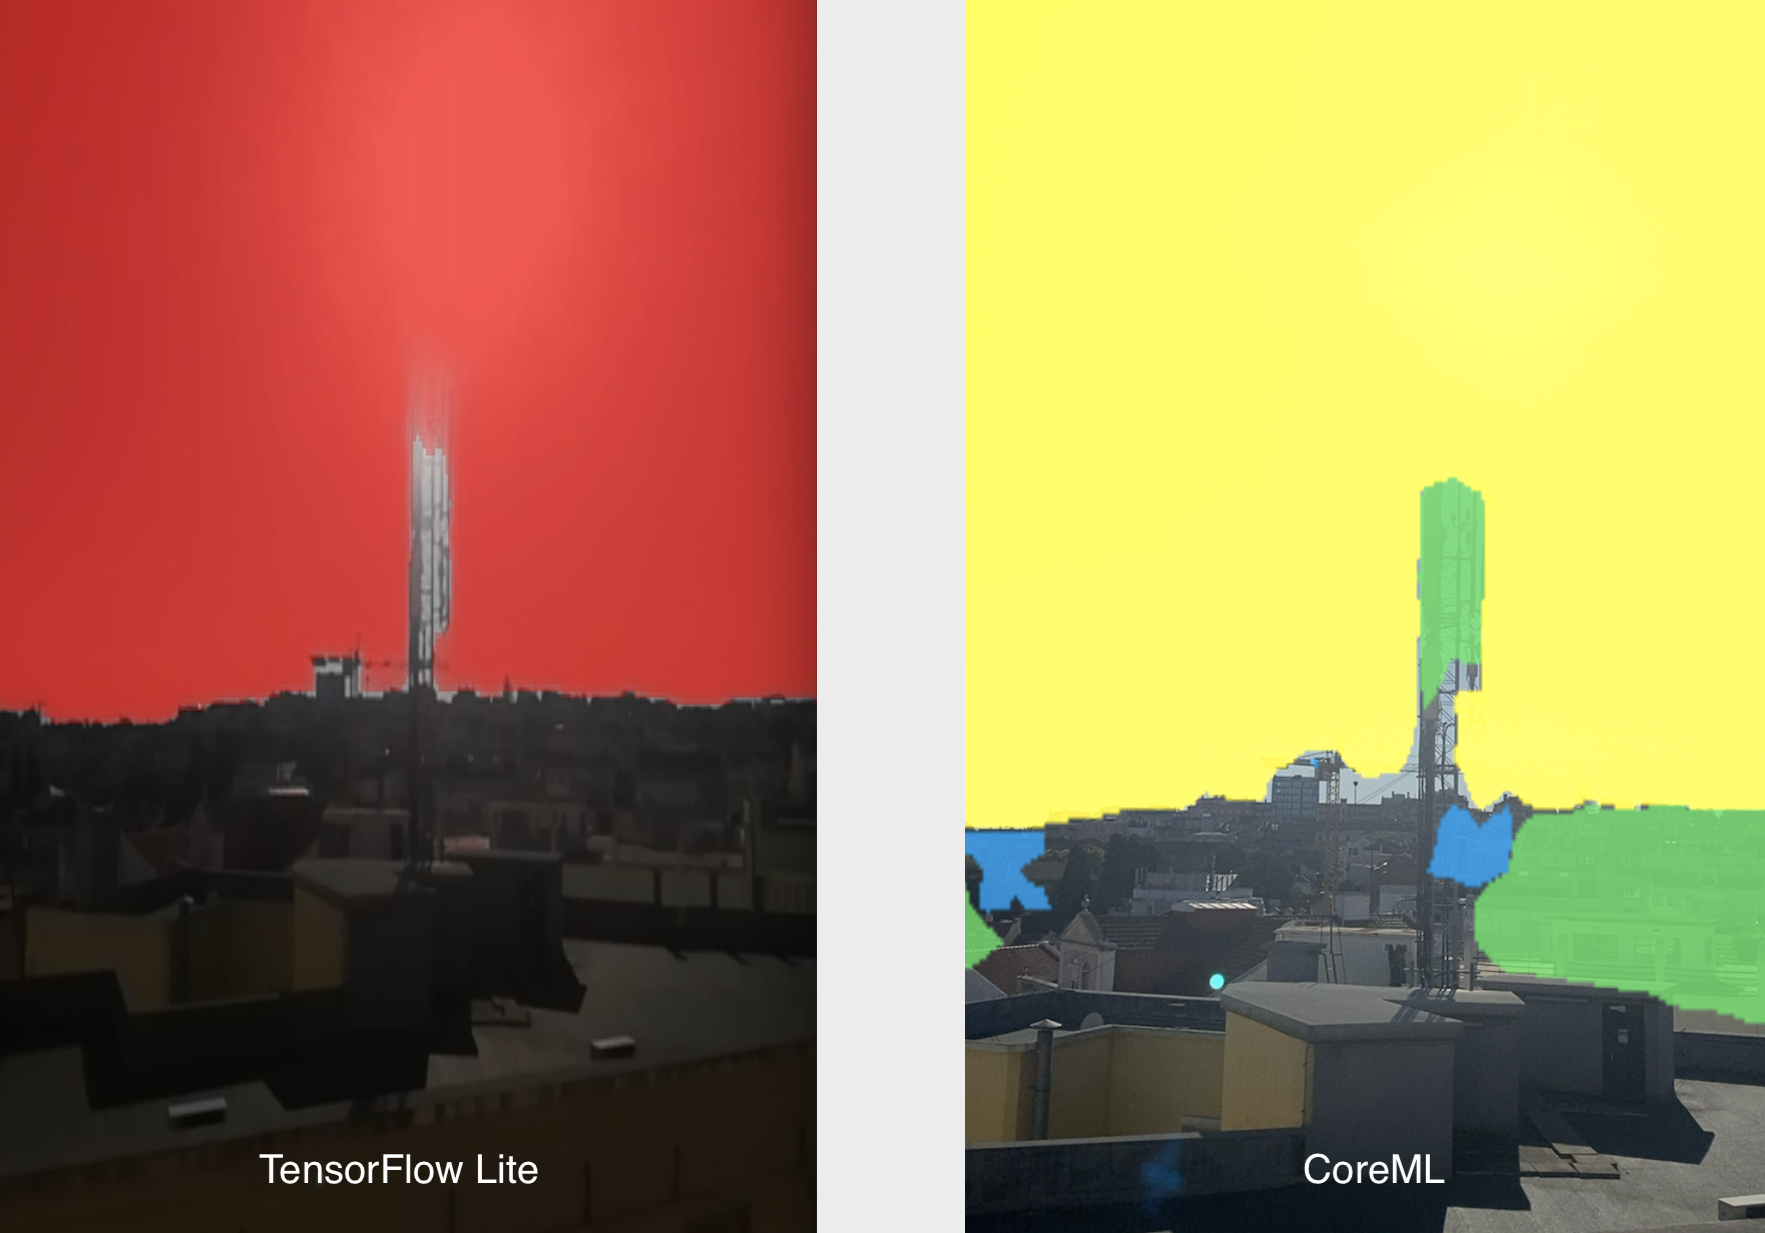
\includegraphics[scale=0.4]{SkySegmentation.png}
	\caption{Test luchtsegmentatie, zonder foutaanduiding}
\end{figure}

De test om de uitkomst van luchtsegmentatie te bekomen werd uitgevoerd in Lissabon in een hotelkamer. Het uitzicht bevat een antenne die de algoritmen een extra moeilijkheid zou kunnen bezorgen bij het uitvoeren van dit experiment, de resultaten zijn dan ook zeer interessant. In de onderstaande foto kan men de foute zones waarnemen, deze worden  aangegeven door middel van de roze zones. Men kan ook alvast opmerken dat de beeldkwaliteit van de camera een grote rol speelt bij dit experiment, de Core. De zeer kleine vlakken tussen de spaken van de antennen zorgen voor foute resultaten. Hieruit kan men bepalen dat het voor beide frameworks moeilijk is om zeer kleine vlakken te koppelen aan een bepaald segment. Dit visueel redeneringsproces werd ook 29 maal herhaald, en ook hier werd een puntensysteem gebruikt om de eindwinnaar te bepalen. In elke test kreeg het framework met het minste aantal foute zones een punt, het framework met het meeste punten na de 29ste test werd bekroond als 'winnaar' van dit deelexperiment. Uit de resultaten van dit deelexperiment kan men dus verder bepalen of de frameworks voldoen aan de nodige aspecten op vlak van nauwkeurig -en correctheid..
\begin{figure}[H]
	\centering
	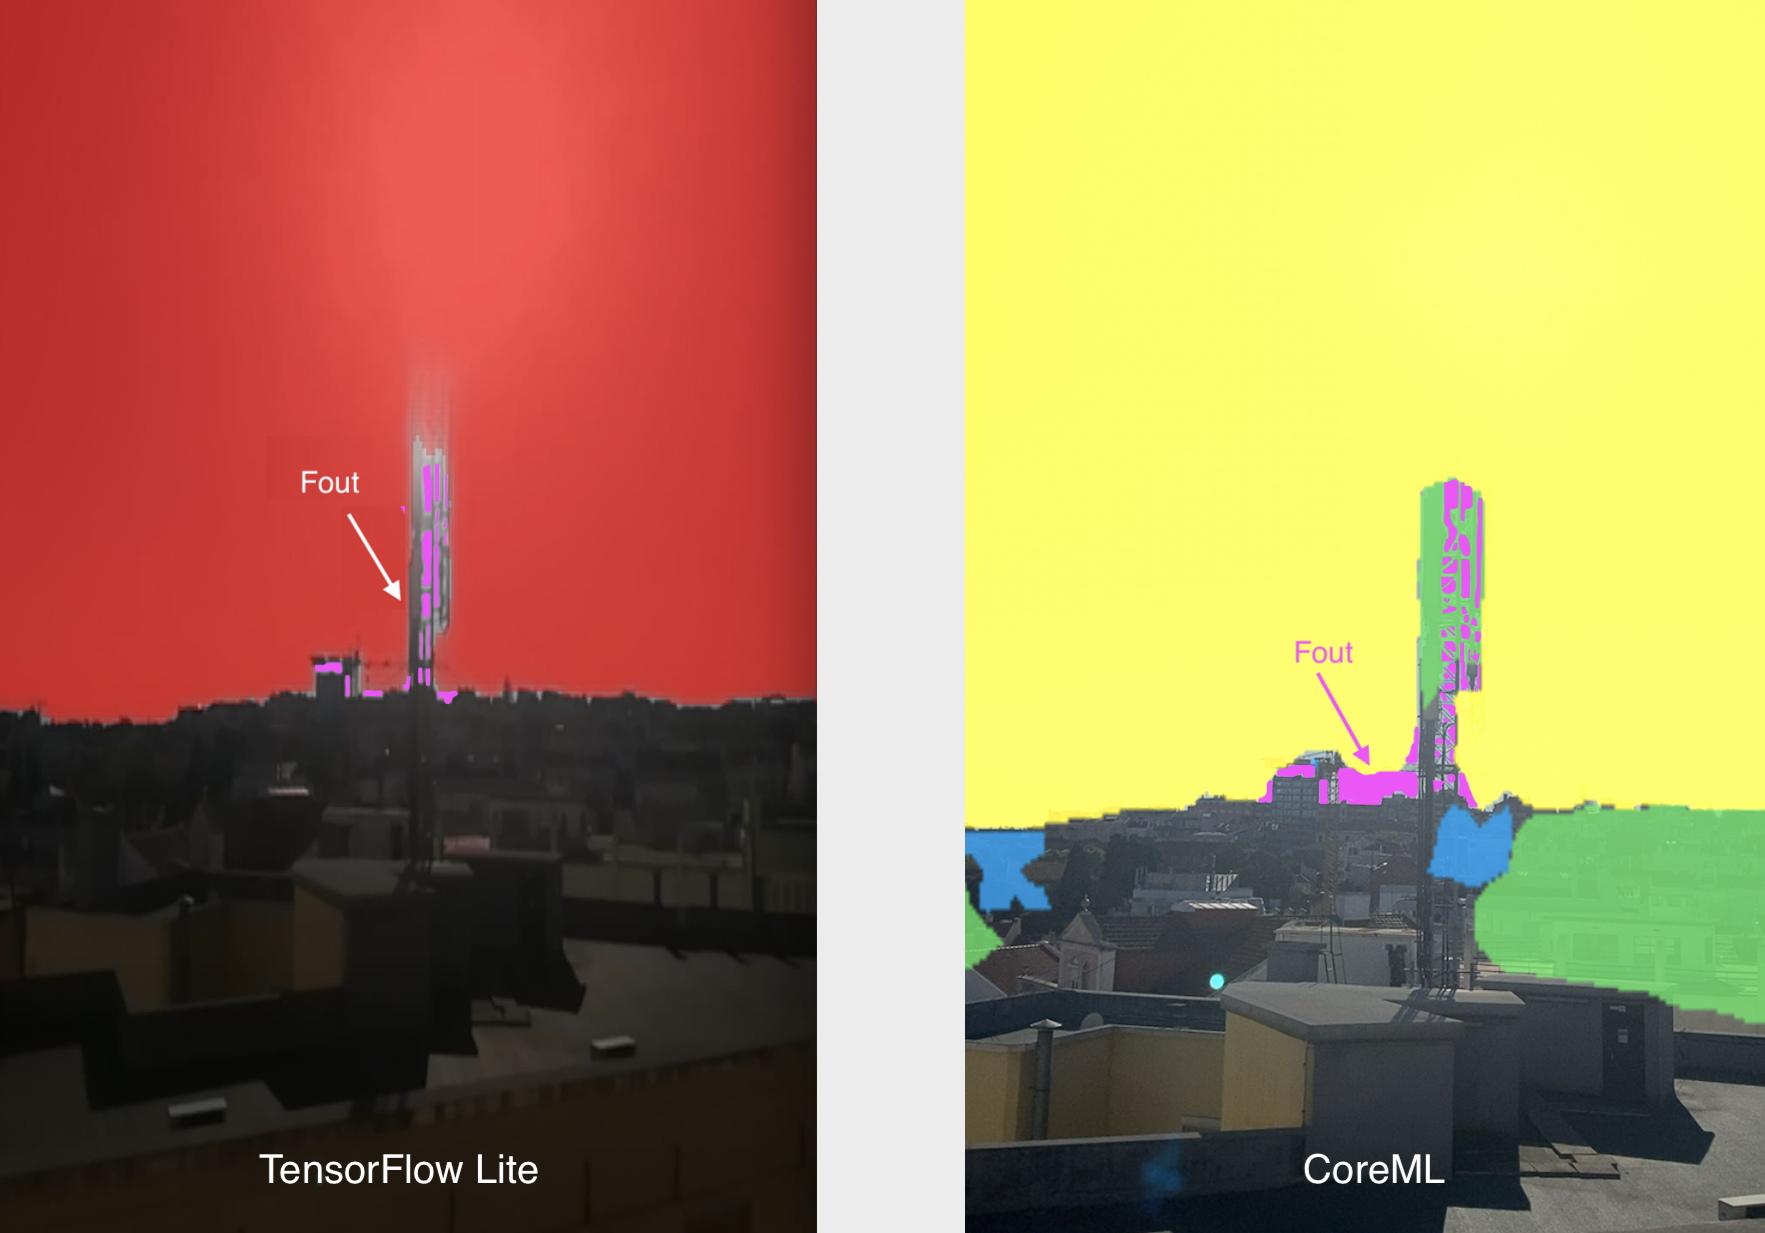
\includegraphics[scale=0.4]{SkySegmentation_MetFoutAanduiding.png}
	\caption{Test luchtsegmentatie, met foutaanduiding}
\end{figure}


\subsection{Segmentatie binnen gebouwen}
Segmentatie binnen gebouwen is de AI-eigenschap die het meeste zal doorwegen in het bepalen van het eindresultaat. De informatie die men uit dit experiment kan vergaren leunt het dichtste bij wat men nodig heeft om de wayfinding context te optimaliseren. Ten eerste is het zeer interessant om te zien hoe de AI-frameworks zullen reageren op de experimenten. Ten tweede is het ook zeer belangrijk om te weten of de bepaalde frameworks de muren of vloer binnen de opgegeven ruimte kan ontdekken + aanduiden. 

Tijdens het exploratief onderzoek was het niet vanzelfsprekend om twee uitgewerkte voorbeelden (TensorFlow Lite + CoreML) te vinden die gebruik maakten van dezelfde dataset. Daarom is het  experiment als volgt te werk gegaan, men testte twee uitgewerkte voorbeelden die elk een verschillende dataset utiliseerden. Men kan deze twee testresultaten dus niet rechtstreeks tegenover elkaar zetten. Alsnog kan men deze vergelijken met elkaar als men evalueert hoe goed beide frameworks in hun opzet zijn geslaagd. Het CoreML-framework werd getest door middel van de 'Fritz AI Studio' applicatie, deze maakt gebruik van een dataset die werd samengesteld door 'Fritz AI', de applicatie zal de volledige ruimte in kaart proberen brengen door middel van verschillende kleurvlekken. TensorFlow Lite werd getest door de 'Tiramisu' applicatie die werd gecreërd door Christian Kauten, deze applicatie is vooral gericht op het herkennen van de grond. Beide tests werden uitgevoerd met een iPhone 11. (camera: 12MP). 

Om deze AI-eigenschap zo optimaal mogelijk te evalueren heeft men beide frameworks getest op 3 verschillende plaatsen, deze plaatsen werden eerder aangegeven in Figuur 3.2 in de methodologie.

\subsubsection{Test 1}
\begin{figure}[H]
	\centering
	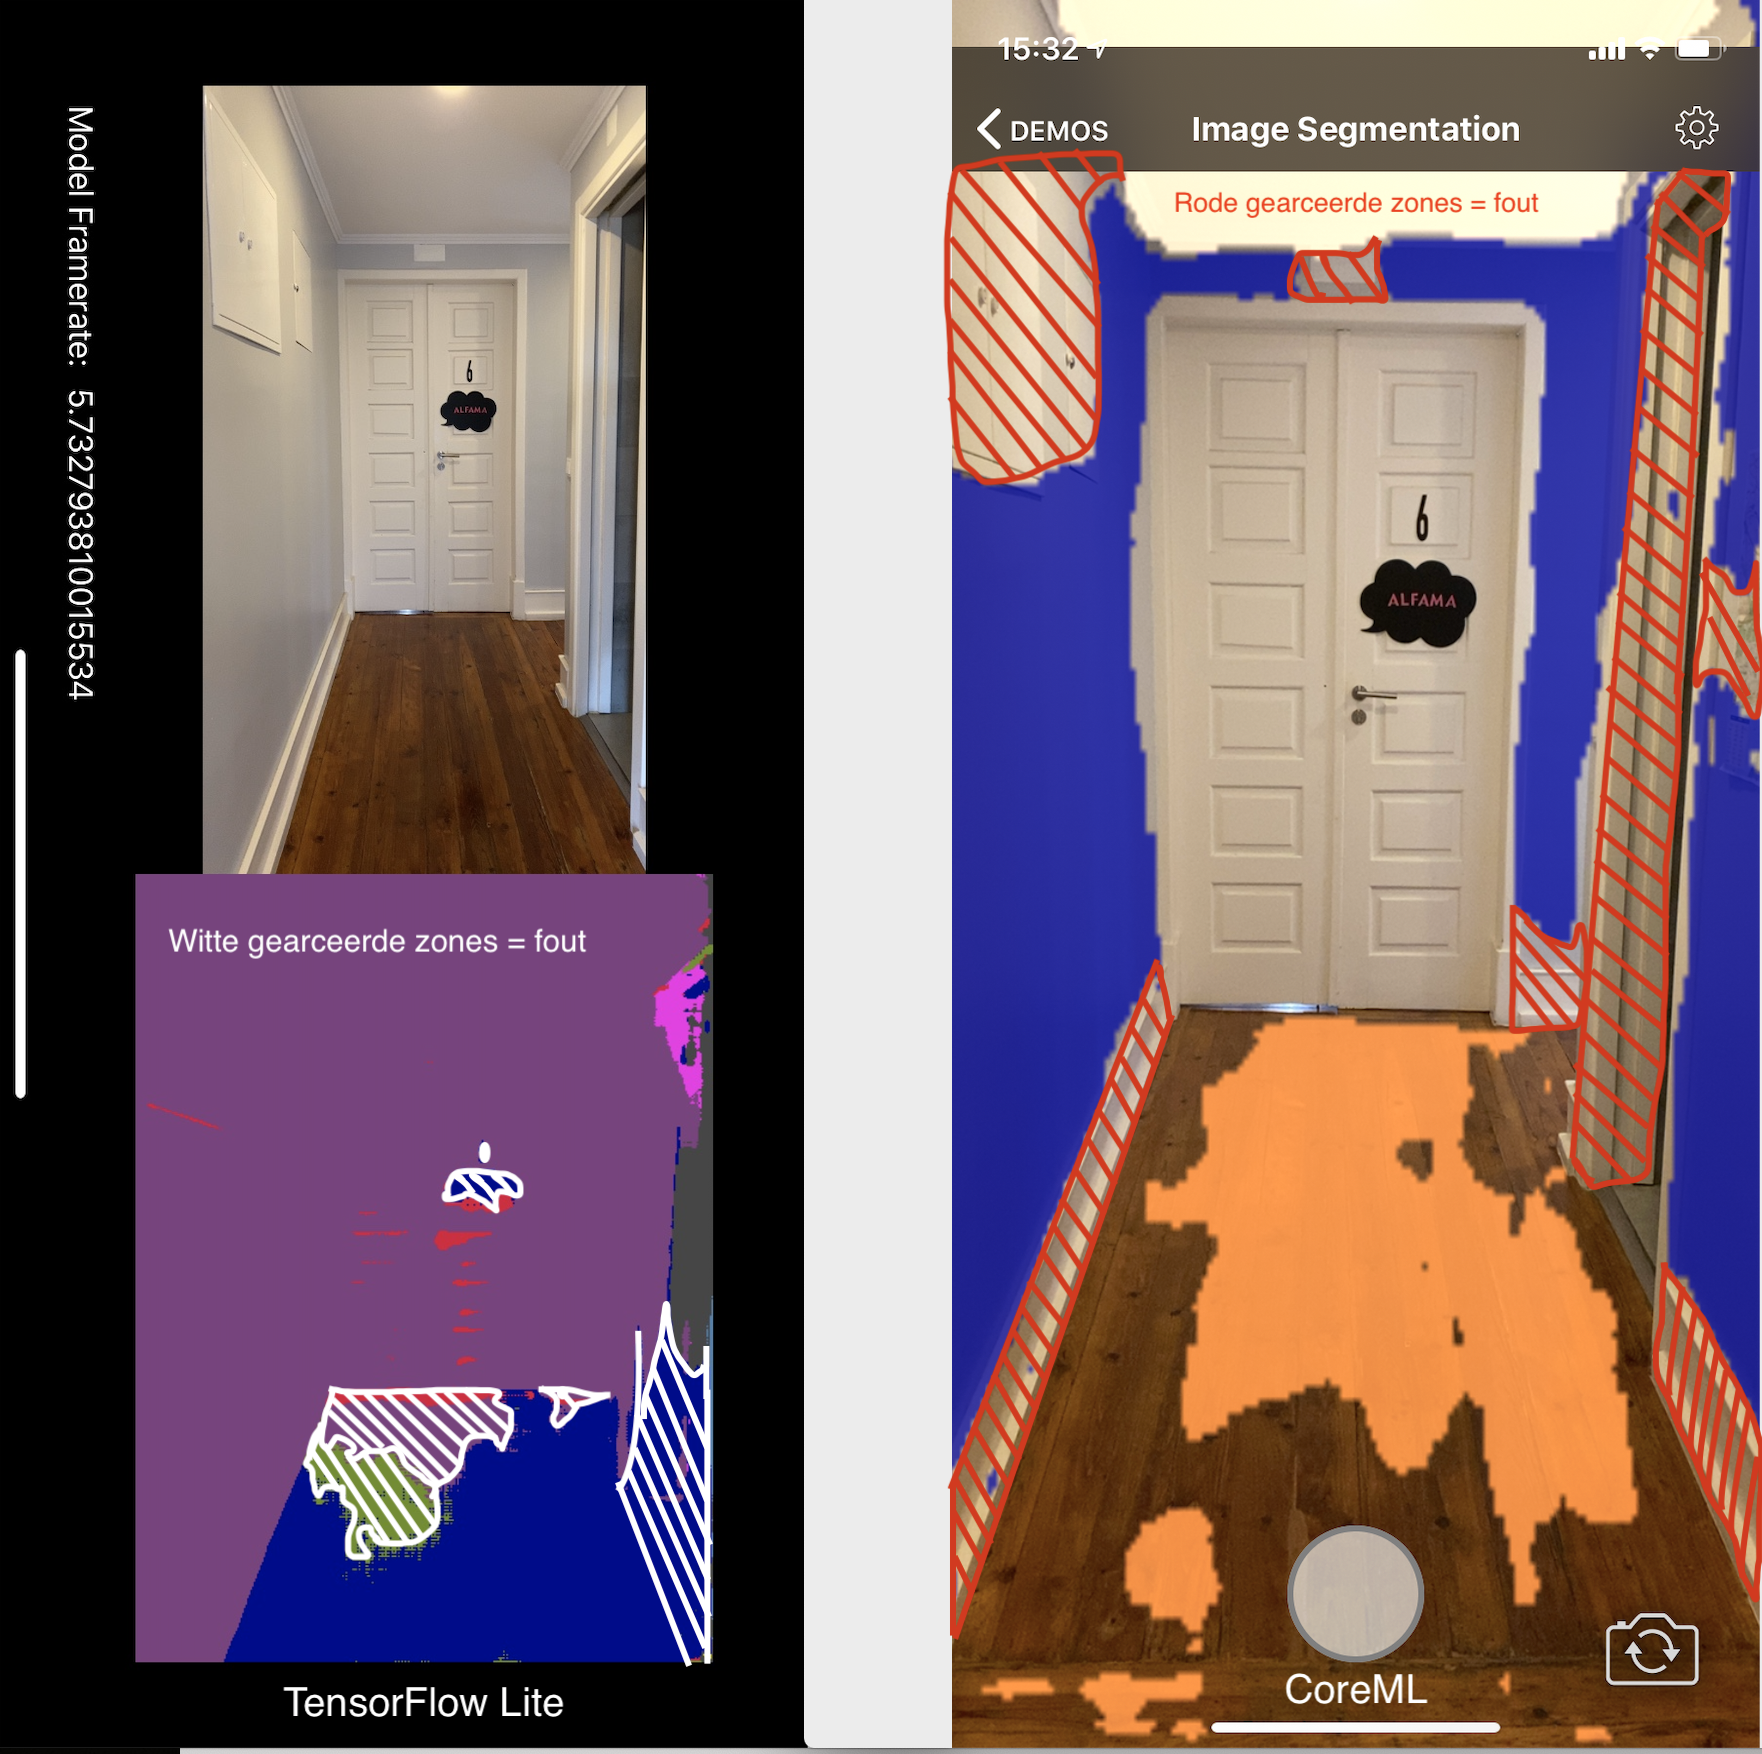
\includegraphics[scale=0.325]{ImageSegmentation_1.png}
	\caption{Test 1: TensorFlow Lite (links) \& CoreML (rechts)}
\end{figure}

De bovenstaande afbeelding toont hoe de eerste test is verlopen. Het TensorFlow Lite-framework zal in deze test zich focussen op het herkennen van grondoppervlaktes, het model is zo getrained. Het CoreML-framework is beter getrained, zoals men kan zien in de bovenstaande afbeelding kan dit framework de grond en muren detecteren, men zal zich voor dit framework vooral focussen op het detecteren van muren, de muurdetectie wordt als extra voordeel beschouwd.

De gearceerde zones (wit voor TensorFlow Lite, rood voor CoreML) tonen aan welke plaatsen men niet kon detecteren, maar wel moesten gedetecteerd worden. Zoals men eerder heeft vermeld worden deze twee tests niet rechstreeks met elkaar vergeleken, als men het aantal gearceerde zones kritiekloos met elkaar zou vergelijken, dan zou dit voor verkeerde resultaten zorgen. Men kan namelijk constateren dat er veel meer muuroppervlaktes zijn dan grondoppervlaktes, de kans dat er dus meer fouten optreden bij het herkennen van de muren is dus groter.

Dit redeneringsproces werd 29 keer herhaald, op deze manier kan men de consistentie van de frameworks testen,  'beginnersgeluk' wordt op deze manier vermeden. In elke iteratie werd gekeken welk framework het beste kon presteren in zijn doelopdracht, voor TensorFlow Lite ging men dus kijken hoeveel grondoppervlakte men kon herkennen, hetzelfde werd bij CoreML gedaan, maar dan met betrekking to muurherkenning. Het framework die het beste kon presteren kreeg in elke iteratie een punt. Na de 29ste iteratie werd gekeken welk framework de meeste punten had.

\subsubsection{Test 2}
\begin{figure}[H]
	\centering
	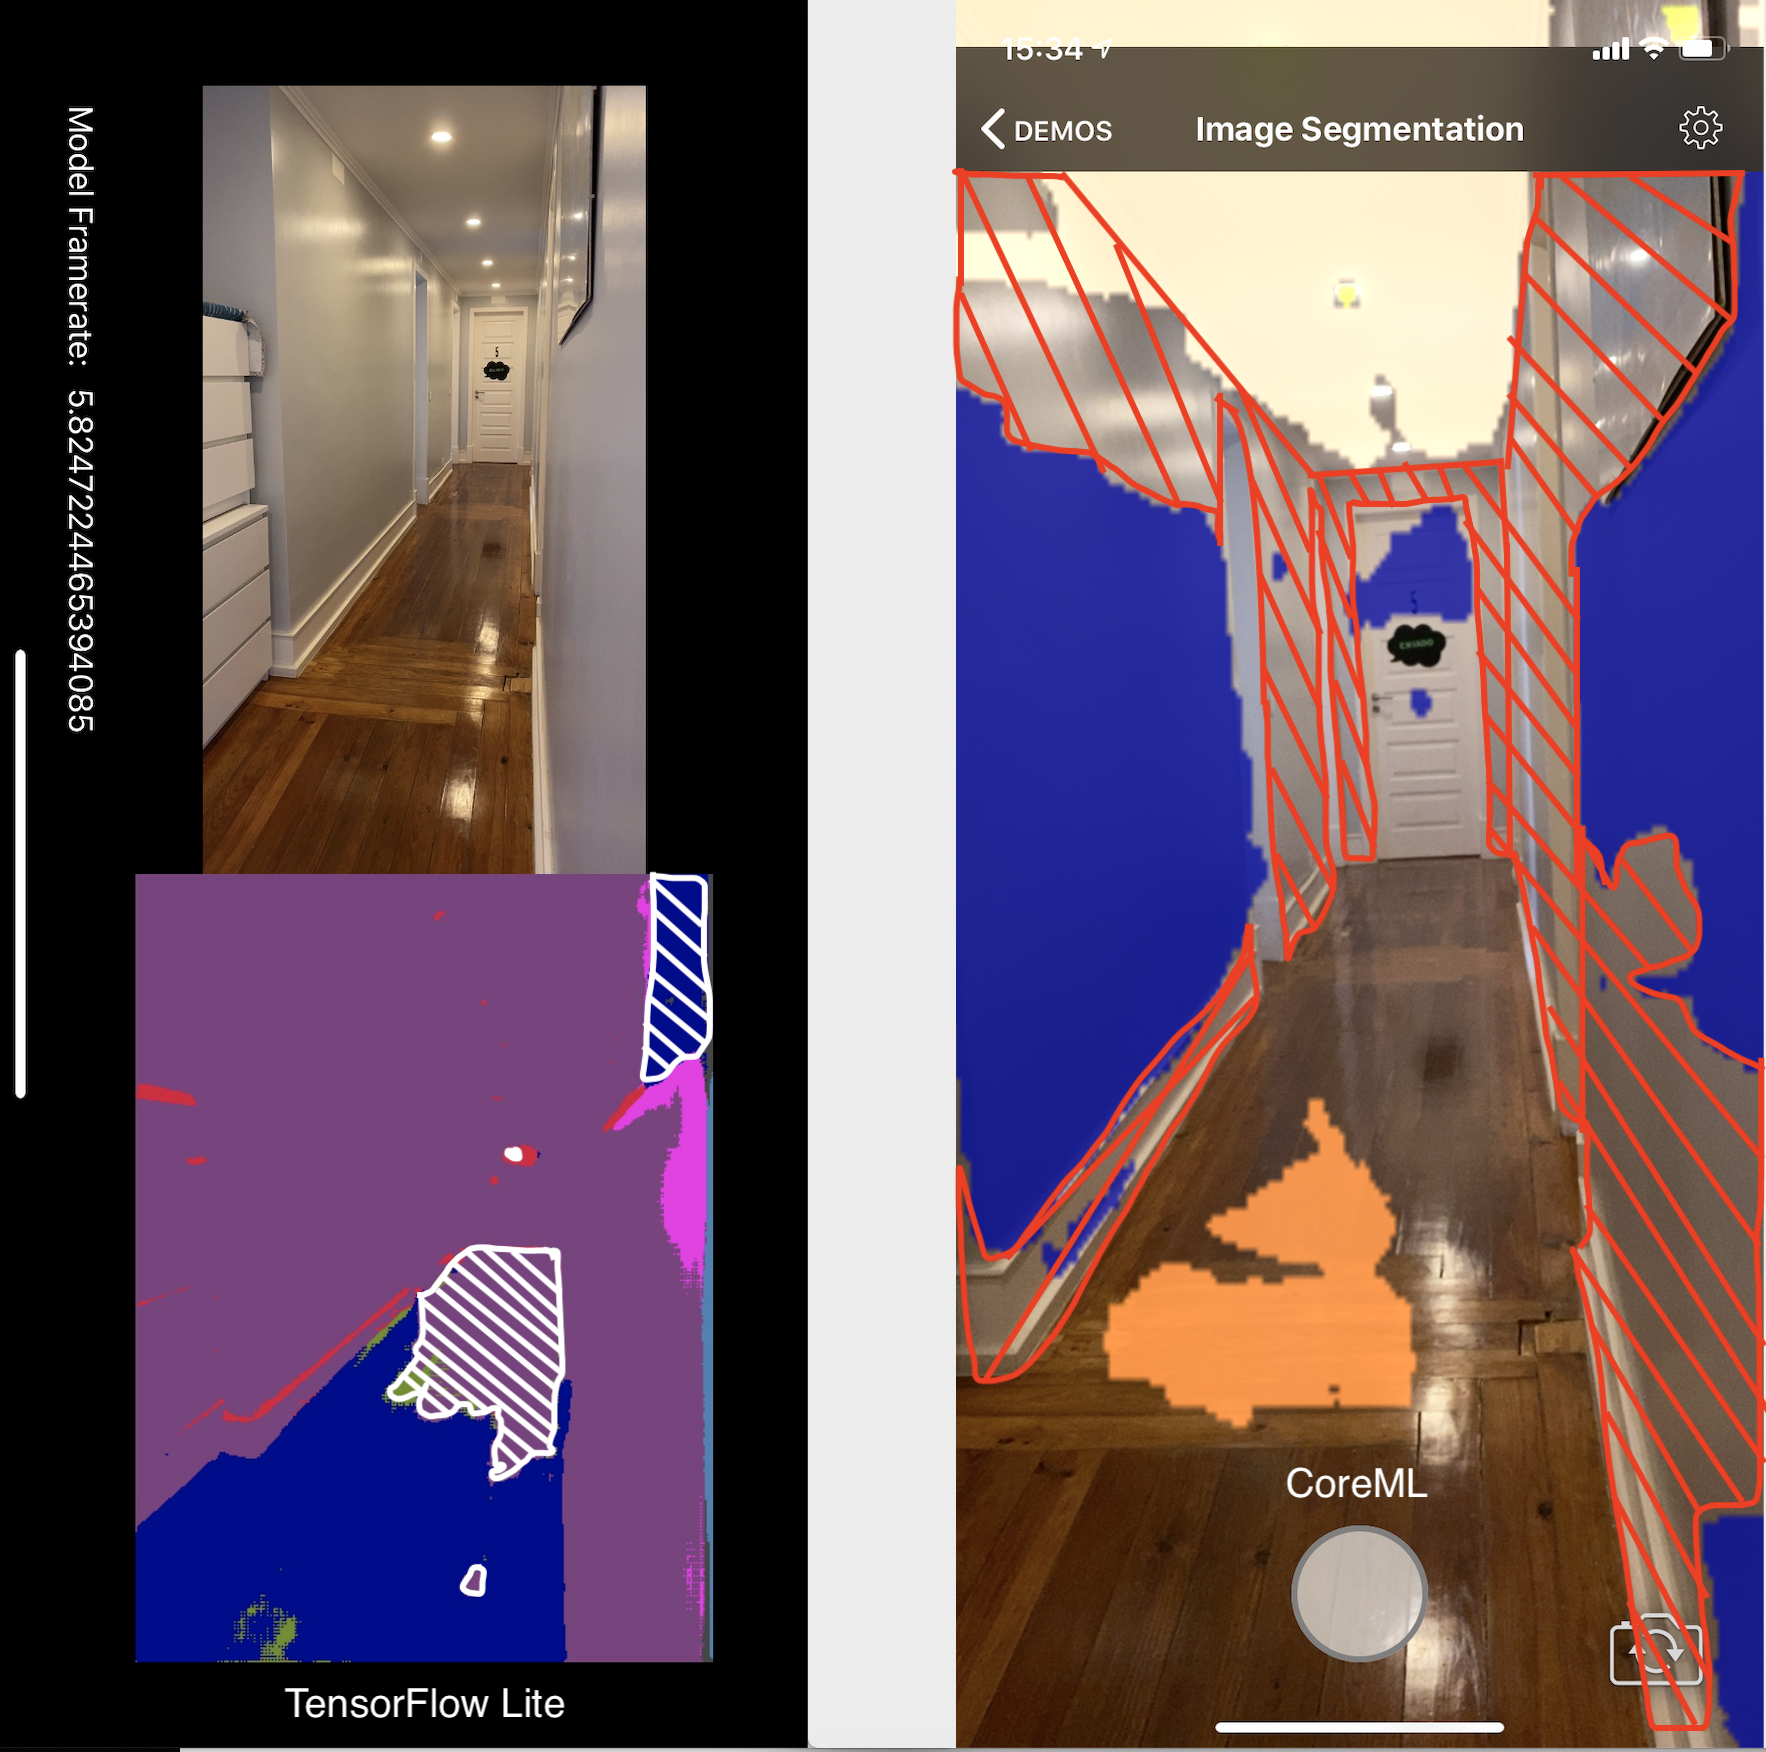
\includegraphics[scale=0.35]{ImageSegmentation_3.png}
	\caption{Test 2: TensorFlow Lite (links) \& CoreML (rechts)}
\end{figure}
De tweede test verliep op dezelfde manier als de eerste (zie bovenstaande foto), alleen de locatie werd gewijzigd. Deze test werd uitgevoerd in een langere gang, op deze manier kon men testen of de frameworks ook het grondoppervlak en de muren kon herkennen die zich verder begeefden. 

Ook in deze test werd er gekeken naar de foute gearceerde zones (wit voor TensorFlow Lite, rood voor CoreML). De regels die werden toegepast in de eerste test werden ook gebruikt in deze test, men kan in dit voorbeeld namelijk ook opmerken dat er veel meer muren aanwezig zijn als grond.

In deze test kan men duidelijk constateren dat het TensorFlow Lite-framework een beter resultaat oplevert als CoreML. CoreML slaagt in de voorbeeld er niet in om het grootste deel van de muren aan te duiden. Dit redeneringsproces werd zoals de andere testen reeds 29 keer herhaald, de evaluatie verliep op dezelfde wijze als de eerste test.

\subsubsection{Test 3}
\begin{figure}[H]
	\centering
	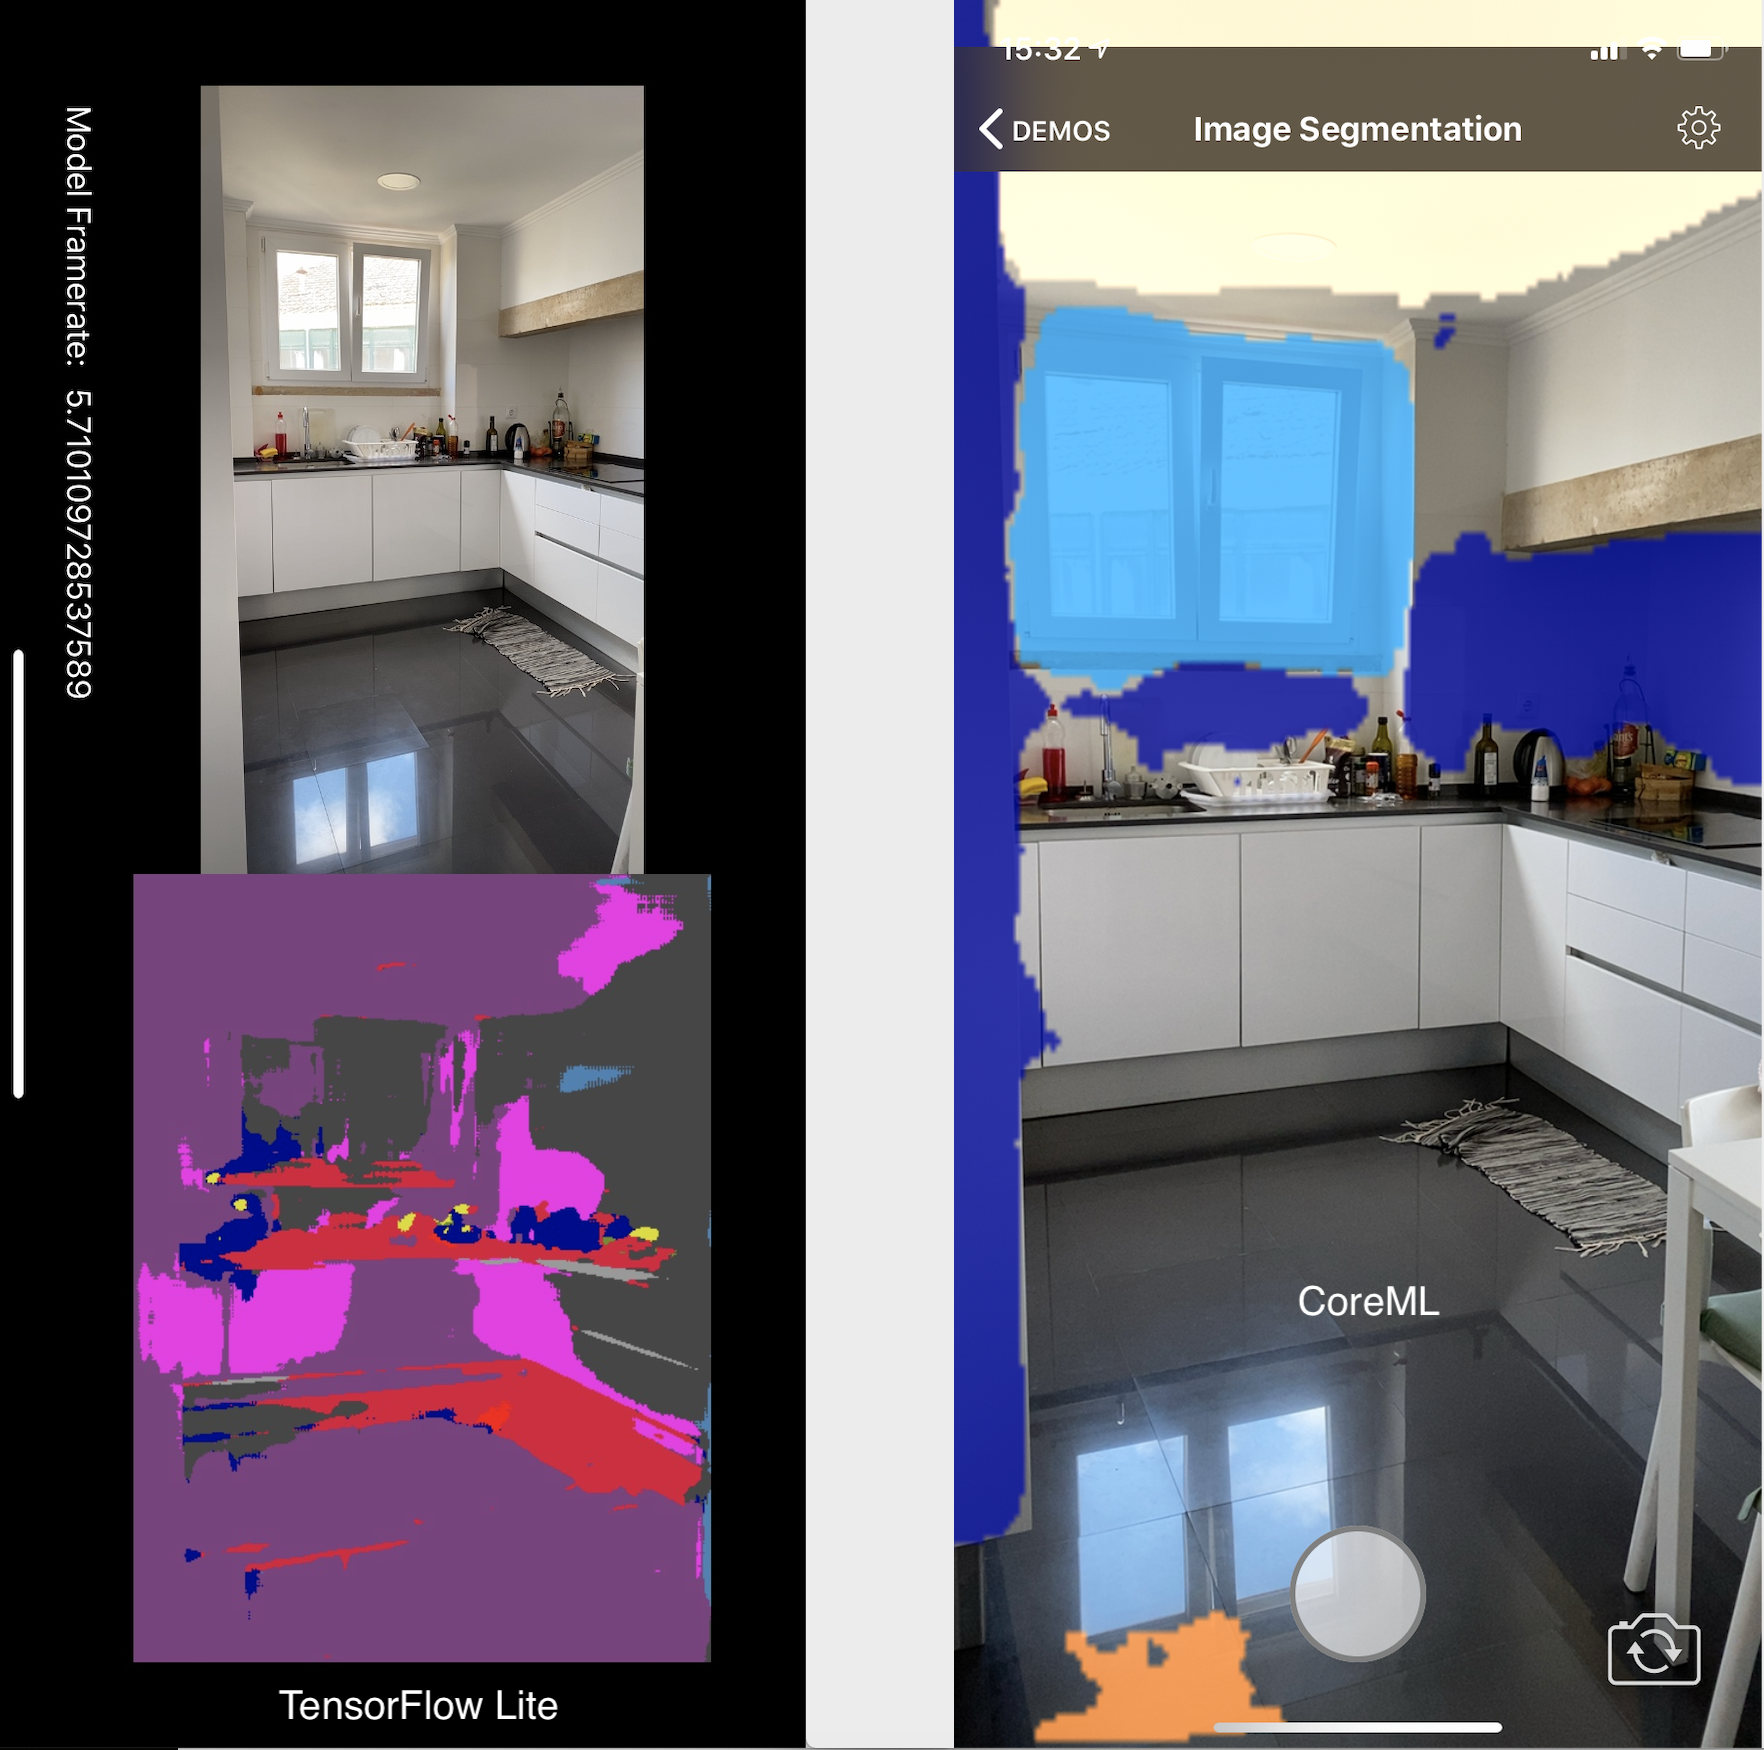
\includegraphics[scale=0.35]{ImageSegmentation_2.png}
	\caption{Test 2: TensorFlow Lite (links) \& CoreML (rechts)}
\end{figure}

Om deze AI-eigenschap op een zo optimaal mogelijk manier te testen werd het derde experiment op een locatie uitgevoerd die niets gemeenschappelijk had met de vorige tests. De derde test werd uitgevoerd in een keuken, deze locatie bevat veel verschillende objecten die voor storing zouden kunnen zorgen. De resultaten in het bovenstaande voorbeeld zijn dan ook opmerkelijk.

Om de resultaten te evalueren werd ook in dit voorbeeld gebruik gemaakt van foute zones die werden aangegeven door gearceerde vlekken. (wit voor TensorFlow Lite, rood voor CoreML). Men kan in dit voorbeeld constateren dat het TensorFlow Lite-framework er helemaal niet in slaagt om de grond te detecteren, een mogelijke factor is het weerkaatsen van het licht in de donkere stenen. Het resultaat van het CoreML-framework kent een beter resultaat, dit framework slaagt er wel degelijk in om de muren grotendeels te detecteren en aan te duiden. Ook deze test werd 29 maal herhaald, de regels uit de vorige twee testen werden hier ook toegepast. In dit voorbeeld zou het CoreML-framework een punt verdienen.

\chapter{\IfLanguageName{dutch}{Resultaten}{Results}}
\label{ch:resultaten}

In dit hoofdstuk zal men de resultaten bespreken van de uitgevoerde testen, dit zal worden gedaan met behulp van grafieken om het overzicht te bewaren. De resultaten zullen eerst worden besproken per AI-eigenschap, op het einde van dit hoofdstuk zal men een algemene conclusie vormen.

\section{Objectdetectie}

\subsection{Test met boek}
De resultaten van de eerste objectdetecttest zijn opmerkelijk, er is namelijk een zeer groot verschil tussen de 2 frameworks. CoreML haalde een gemiddelde van 88.9 \% (standaardafwijking: 10.41) terwijl TensorFlow Lite maar een gemiddelde haalde van 53.83 \% (standaardafwijking: 3.41), dit wilt zeggen dat het TensorFlow Lite-framework slechts in 53 van de 100 gevallen het boek correct zal herkennen en detecteren. Men kan wel constateren dat het CoreML-framework minder consistent is, de verschillende metingen zijn namelijk heel verpreid.

\begin{figure}[H]
	\centering
	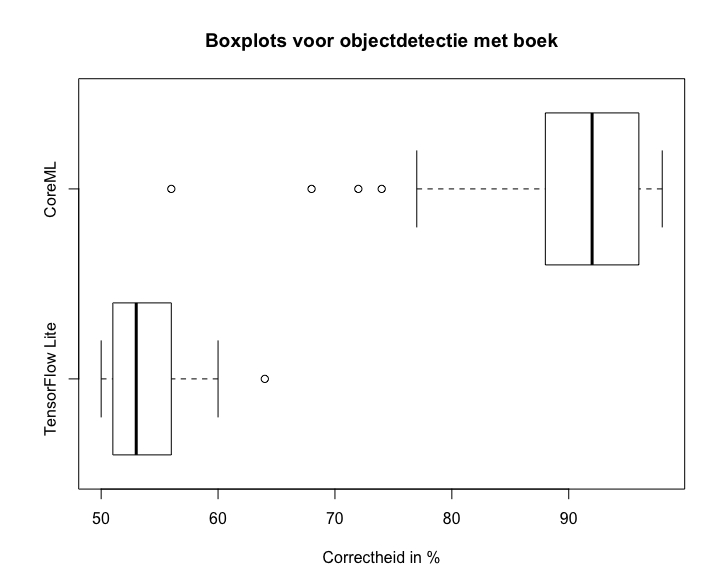
\includegraphics[scale=0.38]{Boxplots_Boek.png}
	\caption{Boxplots test boek}
\end{figure}
\subsection{Test met persoon}

De tweede test bracht eveneens zeer opmerkelijke resultaten, in de onderstaande boxplot kan men opmerken dat het CoreML-framework in bijna alle gevallen de persoon in kwestie met 100 \% zekerheid kon aanduiden. Het framework dat door TensorFlow wordt aangeboden scoort hier ook goed met een gemiddelde van 80 \% (standaardafwijking: 2.51). CoreML haalde in deze test een gemiddelde van 99.78 \% (standaardafwijking: 0.42), de lage waarde voor de standaardafwijking vertaalt zich in een zeer goede consistentie.
\begin{figure}[H]
	\centering
	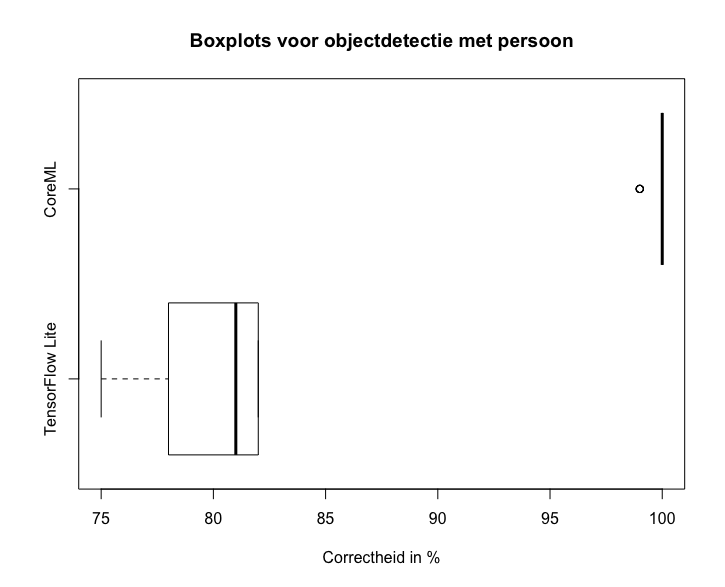
\includegraphics[scale=0.4]{Boxplots_Persoon.png}
	\caption{Boxplots test persoon}
\end{figure}

\subsection{Test met fles}
De derde zorgde voor gelijkaardige resultaten als de vorige tests. Opnieuw presteerde het CoreML-framework veel beter als TensorFlow Lite. Het framework van apple haalde een gemiddelde van 91.55 \% (standaardafwijking: 4.52), voor TensorFlow Lite bedraagde dit 58.89 \% (standaardafwijking: 3.65). Men kan andermaal concluderen dat beide frameworks consistente resultaten behaalden, dit is ook visueel zienbaar in de onderstaande boxplots. 
\begin{figure}[H]
	\centering
	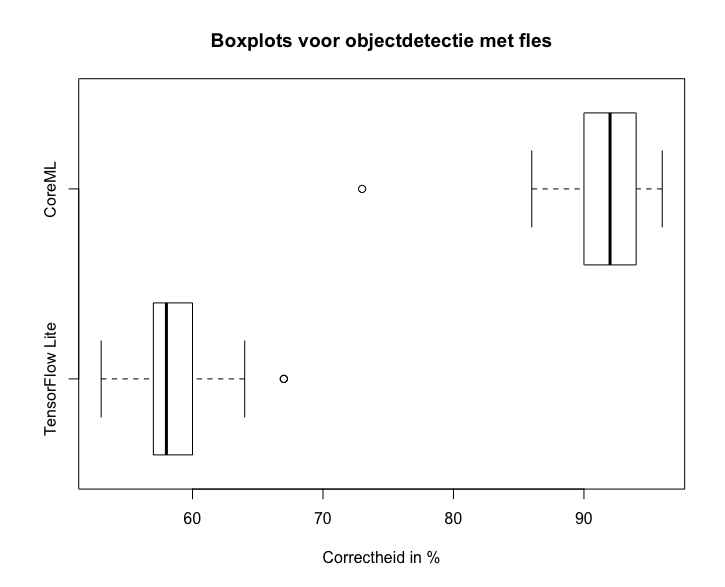
\includegraphics[scale=0.45]{Boxplots_Fles.png}
	\caption{Boxplots test fles}
\end{figure}
\subsection{Test met horloge}
De resultaten uit het vierde experiment zijn zeer interessant, opnieuw scoort het CoreML-framework betere resultaten dan TensorFlow Lite. CoreML haalde een gemiddelde van 78.55 \% (standaardafwijking: 13.38), TensorFlow lite behaalde 66.38 \% (standaardafwijking: 4.39). Op het eerste zicht lijkt CoreML de 'winnaar' in dit experiment, alsnog moet men dit in betwijfeling trekken. De consistentie van CoreML in dit experiment is zeer slecht, de resultaten fluctueren namelijk tussen de  56 en 95 \%. De hoge standaardafwijking is vervolgens ook visueel aantoonbaar op de onderstaande boxplot.
\begin{figure}[H]
	\centering
	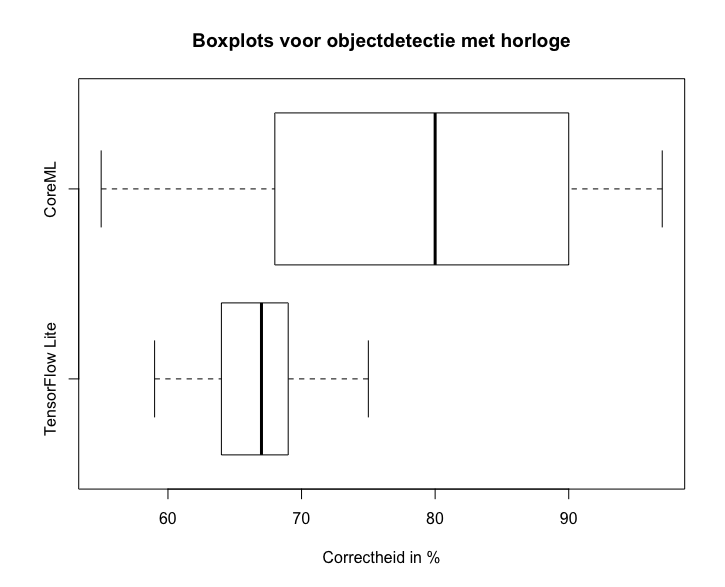
\includegraphics[scale=0.4]{Boxplots_Horloge.png}
	\caption{Boxplots test horloge}
\end{figure}
\subsection{Evaluatie}
In het algemeen kan men besluiten dat het CoreML-framework de beste  resultaten levert op vlak van objectdetectie. Men kan wel concluderen dat de hoge gemiddeldes vaak gepaard gaan met hoge standaardafwijkingen, dit betekent dat de consistentie lager is. In de onderstaande grafiek kan men telkens opnieuw zien dat CoreML ruim beter presteert. Zoals men eerder al heeft vermeld geeft deze AI-eigenschap een beter zicht over de nauwkeurig -en correctheid van het gebruikte algoritme.
\begin{figure}[H]
	\centering
	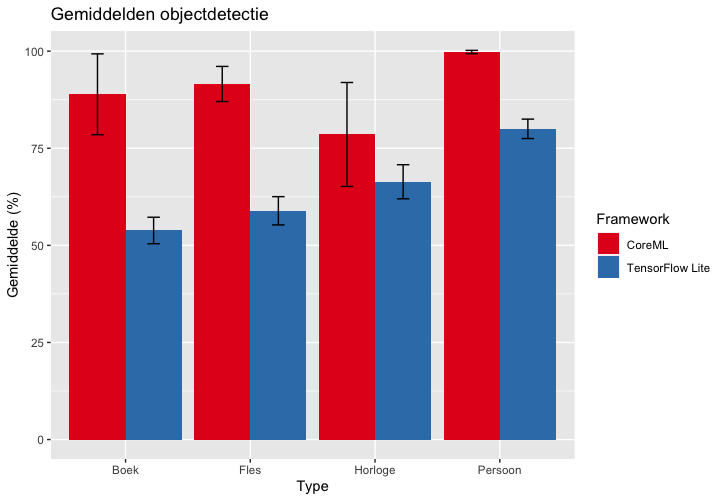
\includegraphics[scale=0.45]{Gemiddelde_objectdetectie.png}
	\caption{Gemiddelden objectdetectie}
\end{figure}

\section{Segmentatie}
\subsection{Menssegmentatie}
\begin{table}[H]
	\centering
	\begin{tabular}{|c|c|c|}
		\hline
		& \textbf{TensorFlow Lite} & \textbf{CoreML} \\ \hline
		\textbf{Aantal punten} & 3                        & 26              \\ \hline
	\end{tabular}
	\caption{Resultaten menssegmentatie test}
\end{table}

De resultaten uit de eerste segmentatietest zijn merkwaardig, CoreML haalt in deze test opnieuw de betere uitkomst. Het framework van Apple wist in 26 van de 29 een betere segmentatie uit zijn mouw te schudden. Het TensorFlow Lite-framework werkte niet nauwkeurig en gaf zeer vaak een compleet verkeerde output, CoreML slaagde er in om bijna elke test met minimale fouten af te werken.

\subsection{Luchtsegmentatie}
\begin{table}[H]
	\centering
	\begin{tabular}{|c|c|c|}
		\hline
		& \textbf{TensorFlow Lite} & \textbf{CoreML} \\ \hline
		\textbf{Aantal punten} & 7                        & 22              \\ \hline
	\end{tabular}
	\caption{Resultaten luchtsegmentatie test}
\end{table}

De tweede test werd op een simultane wijze uitgevoerd als de eerste, ook in deze test kan men zien dat CoreML betere prestaties levert. Men kan wel concluderen dat TensorFlow Lite een betere resultaat haalt als bij menssegmentatie. Alsnog kon men te veel fouten bespeuren in de resultaten van TensorFlow Lite. Bovendien was het CoreML-framework ook in staat om andere objecten binnen de afbeelding te segmenteren, ookal werden beide frameworks op dezelfde manier getrained.
\subsection{Segmentatie binnen gebouwen}

\subsubsection{Korte gang}
\begin{table}[H]
	\centering
	\begin{tabular}{|c|c|c|}
		\hline
		& \textbf{TensorFlow Lite} & \textbf{CoreML} \\ \hline
		\textbf{Aantal punten} & 3                        & 26              \\ \hline
	\end{tabular}
	\caption{Resultaten segmentatie binnen gebouwen: korte gang}
\end{table}
Zoals men eerder had beschreven werd de segmentatie binnen gebouwen op drie verschillende plaatsen getest. De resultaten van de eerste test zijn opnieuw zeer interessant. Opnieuw kan men significant verschil opmerken, het CoreML-framework slaagt er terug in om de beste resultaten te behalen. Ook tijdens het uitvoeren van de test kon men opmerken dat TensorFlow Lite een grondoppervlakt detecteerde die er in de werkelijkheid niet was, deze fouten zorgde voornamelijk voor het grote puntenverschil.

\subsubsection{Lange gang}
\begin{table}[H]
	\centering
	\begin{tabular}{|c|c|c|}
		\hline
		& \textbf{TensorFlow Lite} & \textbf{CoreML} \\ \hline
		\textbf{Aantal punten} & 9                        & 20              \\ \hline
	\end{tabular}
	\caption{Resultaten segmentatie binnen gebouwen: lange gang}
\end{table}
De resultaten van de test in de lange gang zijn ook zeer boeiend, deze test zou beproeven of de frameworks ook het grond -en muuroppervlak zouden detecteren over een langere afstand. Uit de resultaten kan men besluiten dat TensorFlow Lite opnieuw slechter presteert, maar in vergelijking met de vorige test kent men wel een groei. Opnieuw slaagt CoreML beter in zijn opzet, men kon wel een daling zien op vlak van prestaties tegenover de vorige test (in de korte gang).

\subsubsection{Keuken}
\begin{table}[H]
	\centering
	\begin{tabular}{|c|c|c|}
		\hline
		& \textbf{TensorFlow Lite} & \textbf{CoreML} \\ \hline
		\textbf{Aantal punten} & 0                        & 29              \\ \hline
	\end{tabular}
	\caption{Resultaten segmentatie binnen gebouwen: keuken}
\end{table}
In de laatste test kon men opnieuw een gelijkaardig resultaat opmerken. Het TensorFlow Lite slaagt in deze test er helemaal niet in om de grond te detecteren, een weerspiegeling in het grondoppervlak zorgde voor storing. De frameworks moeten in verschillende situaties op dezelfde manier werken, de slechte resultaten zorgden dus zeker voor een 'afstraffing'. Het CoreML-framework slaagde zeker in zijn opzet, het kon de muren bijna perfect detecteren, alsook de grond werd op een goede manier  herkent en gedetecteerd.

\subsection{Evaluatie}
In het algemeen kan men concluderen dat CoreML een veel betere resultaat levert als TensorFlow Lite op vlak van segmentatie. Over de verschillende testen heen kan men telkens zien dat CoreML de hogere punten haalt, het maakte veel minder fouten in het segmenteren van de verschillende objecten, dit kan men visueel ook zien in de onderstaande grafiek. Het TensorFlow Lite-framework is niet nauwkeurig genoeg en vervolgens ook niet bestemd om de omgeving op een optimale manier in kaart te brengen.
\begin{figure}[H]
	\centering
	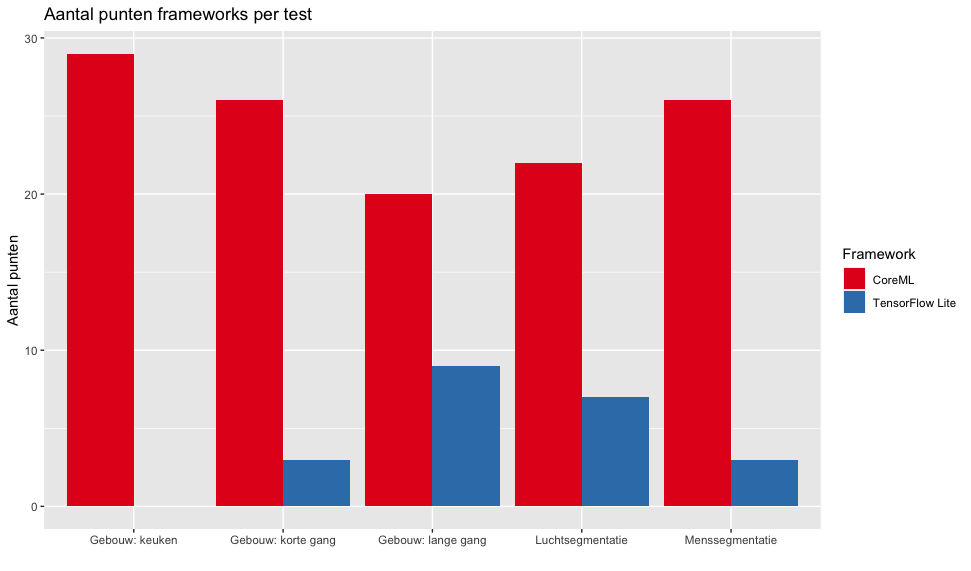
\includegraphics[scale=0.45]{Segmentatie_grafiek.png}
	\caption{Aantal punten per segmentatietest}
\end{figure}

\section{Algemene evaluatie}
Als men alle resultaten naast elkaar plaatst, dan kan men een significant verschil opmerken tussen de twee frameworks. In geen enkele test scoorde TensorFlow Lite beter als CoreML, hieruit kan men besluiten dat CoreML nauwkeuriger, consistener en betrouwbaarder is om te gebruiken als framework voor een wayfinding applicatie. 

In de wayfinding context is het namelijk zeer belangrijk dat men in verschillende situaties een goed zicht of plan van de kamer kan opstellen, dit aspect wordt reeds gedaan door het SLAM-aspect binnen het AR-mechanisme, maar hierin worden nog steeds fouten geconstateerd, om dit te optimaliseren zal men gebruik maken van CoreML.



% Voeg hier je eigen hoofdstukken toe die de ``corpus'' van je bachelorproef
% vormen. De structuur en titels hangen af van je eigen onderzoek. Je kan bv.
% elke fase in je onderzoek in een apart hoofdstuk bespreken.

%\input{...}
%\input{...}
%...

%%=============================================================================
%% Conclusie
%%=============================================================================

\chapter{Conclusie}
\label{ch:conclusie}

% TODO: Trek een duidelijke conclusie, in de vorm van een antwoord op de
% onderzoeksvra(a)g(en). Wat was jouw bijdrage aan het onderzoeksdomein en
% hoe biedt dit meerwaarde aan het vakgebied/doelgroep? 
% Reflecteer kritisch over het resultaat. In Engelse teksten wordt deze sectie
% ``Discussion'' genoemd. Had je deze uitkomst verwacht? Zijn er zaken die nog
% niet duidelijk zijn?
% Heeft het onderzoek geleid tot nieuwe vragen die uitnodigen tot verder 
%onderzoek?

Dit onderzoek heeft aangetoond dat het vinden van het gepaste AI-framework voor een wayfinding context niet vanzelfsprekend is, er is namelijk weinig onderzoek gedaan omtrent de samenwerking van AI en AR-frameworks. De 'jonge' leeftijd van deze technologieën speelt hier parte, zoals eerder werd vermeld werden deze pas in 2017 vrijgegeven. Dit heeft als gevolg dat complexere uitwerkingen nog niet hun optimum hebben bereikt.

Om de AI-kant van dit onderzoek te evalueren werden verschillende tests uitgevoerd op frameworks die werden geselecteerd volgens verscheidene criteria, deze waren gericht op de verschillende AI-eigenschappen die meer info gaven over de correctheid van elk framework. Om deze frameworks zo optimaal mogelijk te testen werden de proeven op verschillende plaatsen uitgevoerd, ook werd er rekening gehouden met consistentie. De consistentie werd beproeft door elke  test op een iteratieve wijze uit te voeren. Het aantal iteraties werd ook zorgvuldig gekozen, door een oneven getal te nemen werden ex aequo's vermeden.

De resultaten van het onderzoek stemden niet overeen met de verwachtingen uit het literatuuronderzoek. TensorFlow heeft een goede reputatie binnen de AI-wereld, maar in dit onderzoek voldeed het niet aan zijn normen. CoreML scoorde dan wel beter als verwacht, in sommige testen kon het framework een voorwerp met bijna 100 \% zekerheid aanduiden.
Uit de resultaten van deze tests was er al snel een verband waarneembaar , telkens scoorde CoreML beter dan TensorFlow Lite. 

%Om de werking tussen ARKit en het CoreML-framework verder te onderzoeken werd er ook een minimalistische uitwerken gerealiseerd met Xcode. Uit deze proof of concept kan men concluderen dat het CoreML-framework in staat is om een op goede manier te communiceren met de visuele kant van de applicatie. Men is er zich van bewust dat deze proof of concept niet in direct verband staat met de wayfinding applicatie, deze uitwerking zou kunnen geoptimaliseerd worden door een applicatie te realiseren die hier meer mee in verband staat.

Uit dit onderzoek kan er dus geconcludeerd worden dat CoreML een geschikt AI-framework is voor de uitwerking van een wayfinding applicatie. Het beschikt over alle eigenschappen die noodzakelijk zijn om de weg op een correcte manier aan te geven. Er kan niet besloten worden dat CoreML het meest geschikte framework is voor 'In The Pocket', om deze conclusie te maken zouden alle opgegeven frameworks uit de literatuurstudie moeten getest en geëvalueerd worden.

Dit onderzoek kan dus zeker nog verder uitgebreid worden, ten eerste kunnen alle frameworks uit de literatuurstudie getest en geëvalueerd worden volgens de opgegeven beoordelingstechnieken. Ten tweede zouden de testen op meer plaatsen kunnen uitgewerkt worden. Deze mogelijkheid werd beperkt door de verschillende corona-maatregelen die werden opgelegd door de overheid. Ten derde zou CoreML ook beter kunnen worden getest door middel van een proof-of-concept die in direct verband staat met de wayfinding-context, uit deze applicatie is het dan verder mogelijk om tests uit te voeren die veel doelgerichter zijn.

In de toekomst zou deze uitwerking meer in verband kunnen staan met de wayfinding context. Ten laatste kunnen de proeven grootschaliger worden getest, in plaats van 29 iteraties zou je dit kunnen uitbreiden naar 299. Deze uitwerking zou een beter beeld geven over de consistentie van elke AI-eigenschap.

%%=============================================================================
%% Bijlagen
%%=============================================================================

\appendix
\renewcommand{\chaptername}{Appendix}

%%---------- Onderzoeksvoorstel -----------------------------------------------

\chapter{Onderzoeksvoorstel}

Het onderwerp van deze bachelorproef is gebaseerd op een onderzoeksvoorstel dat vooraf werd beoordeeld door de promotor. Dat voorstel is opgenomen in deze bijlage.

% Verwijzing naar het bestand met de inhoud van het onderzoeksvoorstel
%---------- Inleiding ---------------------------------------------------------
\section{Introductie} % The \section*{} command stops section numbering
\label{sec:introductie}
\subsection{Probleemstelling en context}
Om zich te verplaatsen heeft men reeds smartphones met GPS implementaties, wayfinding is hier het toegepaste voorbeeld. Wayfinding is een toepassing om de gewenste locatie en gerichte informatie te vinden met behulp van omgevingsfactoren, het wordt vooral binnen gebruikt. In The Pocket is een bedrijf dat zich focust op digitale producten, zij wensen een applicatie te implementeren dat wayfinding optimaliseert, dit betekent dat er geen fouten meer worden gemaakt bij het wijzen van de weg. 
Om deze toepassing te optimaliseren verlangt men gebruik te maken van AI en AR om omgevingsfactoren te detecteren en te analyseren, bovendien kan men de input vertalen naar de AR omgeving. Als men bijvoorbeeld tegen een muur dreigt te lopen, dan kan AI dit corrigeren.
In deze bachelorproef zal ik een onderzoek voeren dat resulteert in een overzicht van verschillende mogelijke algoritmes en/of aanpakken. Deze zal men kunnen toepassen bij het implementeren van de gewenste applicatie.

\subsection{Motivatie en relevantie onderzoek}
\subsubsection{Motivatie}
De technologieën die worden toegepast in deze probleemstelling bevinden zich in grote mate tot mijn interesse. Een grondig onderzoek zal mijn kennis verrijken en helpen in de toekomst. 
\subsubsection{Relevantie}
Men kan concluderen dat een onderzoek omtrent de samenhang van AI en AR  zeker relevant is. Er wordt veel geëxpermimenteerd met deze techonologieën en een onderzoek kan hierbij een bijdrage leveren.

\subsection{Doelstelling en onderzoeksvraag}
\subsubsection{Doelstelling}
De doelstelling van dit onderzoek is om een duidelijk overzicht te creëren van welke algoritmes en/of aanpakken goede prestaties zullen leveren bij het implementeren in de wayfinding context. Goede prestaties kan men vertalen in een applicatie die zonder fouten, de juiste route zal aangeven.
\subsubsection{Onderzoeksvraag}
De centrale vraag in dit onderzoek is: "Welke bestaande technieken bestaan er reeds om aan de hand van AI en AR de drift in wayfinding te optimaliseren". Hoe kunnen we de wereld rondom de gebruiker herkennen, analyseren en bovendien de input op een bruikbare manier vertalen naar de AR omgeving.

%---------- Stand van zaken ---------------------------------------------------

\section{State-of-the-art}
\label{sec:state-of-the-art}
In het hedendaagse leven wordt er veel gepraat over AI en AR, maar dit gaat niet vaak in samenhang met wayfinding.
Uit de literatuurstudie kan ik concluderen dat er reeds weinig onderzoek is gedaan naar dit bepaald onderwerp, wat dit onderzoek alleen maar interessanter maakt.
Het onderzoek ~\citetitle{Pouria2016} ~\autocite{Pouria2016} is een goede inspiratie, men gebruikt namelijk een gelijkaardige methodiek om het product uit te werken, er zal dan ook meerdere keren naar verwezen worden in mijn onderzoek.
Het onderzoek omtrent ~\citetitle{Zhang2017} ~\autocite{Zhang2017}  omvat een merkwaardige manier om objecten te gaan detecteren, deze manier kan gebruikt worden in een 'indoor navigation task', wat zeer relevant is voor mijn toekomstig onderzoek.
~\citetitle{Liang2015} ~\autocite{Liang2015} is een onderzoek dat een performant objectherkenning algoritme biedt, het resultaat van dit onderzoek zal ik met zekerheid verwerken.
In de paper ~\citetitle{Haikun2017}~\autocite{Haikun2017} bespreekt men een wijze van aanpak dat leidt tot een geoptimaliseerd wayfinding ontwerp met goed geplaatste borden, rekening houdend met de mogelijkheid van het maken van fouten tijdens een navigatie. Aangezien dit reeds een uitgewerkt voorbeeld is van wayfinding zal ik hier rekening mee houden.
Ten slotte is het zeer belangrijk bij wayfinding om de positie steeds tot in puntjes te kunnen waarnemen, \citetitle{Motlagh2009} ~\autocite{Motlagh2009} is een onderzoek dat een oplossing biedt voor dit probleem.
 


% Voor literatuurverwijzingen zijn er twee belangrijke commando's:
% \autocite{KEY} => (Auteur, jaartal) Gebruik dit als de naam van de auteur
%   geen onderdeel is van de zin.
% \textcite{KEY} => Auteur (jaartal)  Gebruik dit als de auteursnaam wel een
%   functie heeft in de zin (bv. ``Uit onderzoek door Doll & Hill (1954) bleek
%   ...'')

%---------- Methodologie ------------------------------------------------------
\section{Methodologie}
\label{sec:methodologie}
Ten eerste zal ik een grondig exploratief onderzoek uitvoeren naar de verschillende mogelijkheden betreffende bestaande methodieken en technieken. Deze zal ik samenstellen in een overzicht waar men de details van elke methodiek/techniek kan raadplegen. Ten tweede zal ik voor één methodiek/techniek een proof-of-concept uitwerken in een praktisch voorbeeld, hieruit kan men het effectieve resultaat bemerken.
Het exploratief onderzoek zal ik oplijsten met R (en markdown), waar men een duidelijk overzicht zal hebben van elke methodiek/techniek met zijn eigenschappen.
Om de proof-of-concept te realiseren zal ik gebruik maken van een IOS-applicatie waar ik AR en AI zal samenbundelen in een praktisch voorbeeld.

%---------- Verwachte resultaten ----------------------------------------------
\section{Verwachte resultaten}
\label{sec:verwachte_resultaten}

Bij het uitvoeren van het exploratief onderzoek reken ik erop een vijftal technieken te vinden die voldoen aan de wensen van de wayfinding context.

De behaalde resultaten zullen worden verzameld door het uitvoeren van experimenten met de betrokken algoritmes en/of aanpakken uit de technieken. Een experiment zal bestaan uit een mogelijke simulatie die het AI -gebeuren zal testen, men zal m.a.w. gaan nakijken of het AI mechanimse effectief een obstakel detecteert.

Ik verwacht dat elke techniek een correctheid heeft van minstens 80 \%, dit beketent dat in 80 \% van de gevallen het algoritme een obstakel zal detecteren. Ik verwacht ook een techniek te vinden die grosso modo 95 \% correct is.

\begin{figure}[H]
	\centering
	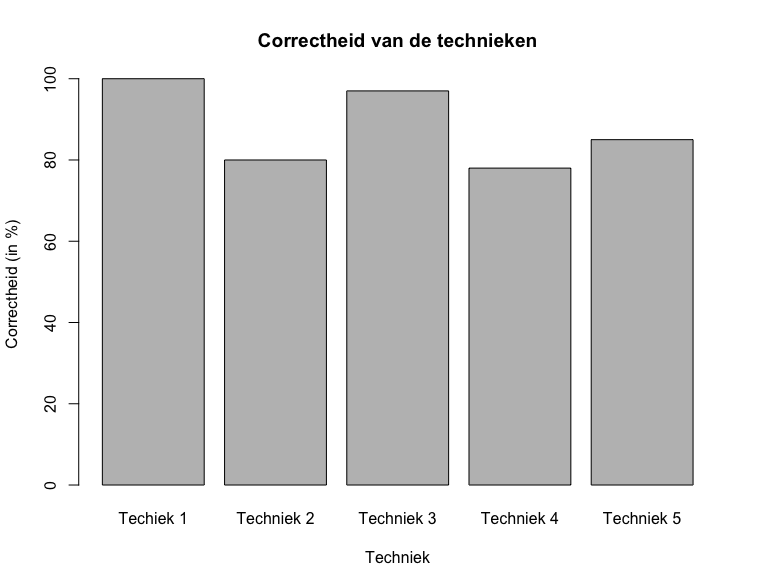
\includegraphics[scale=0.5]{Correctheid_technieken}
	\caption{Verwachte resultaten}
\end{figure}

%---------- Verwachte conclusies ----------------------------------------------
\section{Verwachte conclusies}
\label{sec:verwachte_conclusies}
Door de "jonge leeftijden" van de technoligieën verwacht ik dat het vinden van de nodige documentatie niet van een leien dakje zal lopen, alsook het uitwerken van AI - algoritmes zal zeer complex zijn, maar dit maakt het onderzoek meer uitdagend en zinvol.

Ik hoop een positief resultaat te vinden uit één of meerdere van de experimenten, zodat ik het bedrijf In The Pocket kan helpen bij het vinden van het gepaste algoritme.


%%---------- Andere bijlagen --------------------------------------------------
% TODO: Voeg hier eventuele andere bijlagen toe
%\input{...}

%%---------- Referentielijst --------------------------------------------------

\printbibliography[heading=bibintoc]

\end{document}
